% !TeX root = ../../thesis.tex
\chapter{Appendix to chapter \ref{ch:TranslationSPT}}\label{ch:myappendix}

\section{Representations and states}
In this section we summarize all the results we need from \cite{bratteli1979operator}.
\begin{theorem}\label{thrm:ExistenceGNS}
	Let $\omega$ be a state on a $C^*$-algebra $\AA$. It follows that there exists a cyclic representation $(\HH_\omega,\pi_\omega,\Omega_\omega)$ of $\AA$ such that
	\[\omega(A)=\bra{\Omega_\omega}\ket{\pi_\omega(A)\Omega_\omega}\]
	for all $A\in\AA$. Moreover, the representation is unique up to unitary equivalence.
\end{theorem}
\begin{proof}
	Theorem 2.3.16 in \cite{bratteli1979operator}.
\end{proof}
We will call this cyclic representation a GNS triple for $\omega$.
\begin{corollary}\label{cor:ExistenceOfUnitary}
	Let $\omega$ be a state over the $C^*$-algebra $\AA$ and $\tau$ a *-automorphism of $\AA$ which leaves $\omega$ invariant, i.e.,
	\[\omega\circ\tau=\omega.\]
	Let $(\HH_\omega,\pi_\omega,\Omega_\omega)$ be a GNS triple for $\omega$. It follows that there exists a uniquely determined unitary operator $U_\omega$, such that
	\[U_\omega \pi_\omega(A)U_\omega^\dagger=\pi_\omega\circ\tau(A) \]
	for all $A\in\AA$, and
	\[U_\omega\Omega_\omega=\Omega_\omega. \]
	If furthermore, $\omega$ is pure then (up to a phase) there even exists a unique $U_\omega$ without requiring the second condition.
\end{corollary}
\begin{proof}
	The proof of this corollary is a combination of Corollary 2.3.17 and Theorem 2.3.19 from \cite{bratteli1979operator}.
\end{proof}
The following lemma does not come from Bratteli-Robinson but in stead follows from Wigner's theorem:
\begin{lemma}\label{lem:SplittingOfUnitary}
	Let $\AA$ and $\BB$ be arbitrary unital $C^*$-algebras. Let $(\HH_\AA,\pi_\AA)$ and $(\HH_\BB,\pi_\BB)$ be arbitrary irreducible $*$-representations on $\AA$ and $\BB$ respectively. Let $U\in\UU(\HH_\AA\otimes\HH_\BB)$ be such that there exists an $\alpha_\AA\in\Aut{\AA}$ and an $\alpha_\BB\in\Aut{\BB}$ satisfying
	\begin{equation}
	\Ad{U}\circ(\pi_\AA\otimes\pi_\BB)=\pi_\AA\circ\alpha_\AA\otimes\pi_\BB\circ\alpha_\BB
	\end{equation}
	then there exists a $U_\AA\in\UU(\HH_\AA)$ and a $U_\BB\in\UU(\HH_\BB)$ such that
	\begin{equation}
	U=U_\AA\otimes U_\BB.
	\end{equation}
\end{lemma}
\begin{proof}
	From the assumptions we see that $\forall A\in\AA$
	\begin{equation}
	\Ad{U}\circ\pi_\AA\otimes\pi_\BB(A\otimes\id)=\pi_\AA\circ\alpha_\AA(A)\otimes\id\subset \BB(\HH_\AA)\otimes\id.
	\end{equation}
	Since $\Ad{U}$ is continuous in weak operator topology (on $\BB(\HH_{\AA}\otimes\HH_{\BB})$), it follows that we can extend the map
	\begin{equation}
	\Ad{U}|_{\textrm{Im}(\pi_\AA)}:\textrm{Im}(\pi_\AA)\otimes\id\rightarrow \BB(\HH_\AA)\otimes\id
	\end{equation}
	to the closure in weak operator topology. By irreducibility (and Von Neumanns bicomutant theorem), we get that $\pi_\AA(\AA)''=\BB(\HH_\AA)$ and therefore we get a map
	\begin{equation}
	\Ad{U}|_{\BB(\HH_\AA)\otimes\id}:\BB(\HH_\AA)\otimes\id\rightarrow \BB(\HH_\AA)\otimes\id.
	\end{equation}
	By restriction this gives rise to an automorphism $\tau_\AA:\UU(\HH_\AA)\rightarrow\UU(\HH_\AA)$. By Wigners theorem any automorphism of $\BB(\HH_\AA)$ is inner and therefore there exists a $U_\AA$ such that $\tau_\AA=\Ad{U_\AA}$. Doing the same on $\BB$ gives us similarly a $\tau_\BB$ and a $U_\BB$. We now get
	\begin{equation}
	\Ad{U}\circ(\pi_\AA\otimes\pi_\BB)=\tau_\AA\circ\pi_\AA\otimes\tau_\BB\circ\pi_\BB=\Ad{U_\AA\otimes U_\BB}\circ(\pi_\AA\otimes\pi_\BB).
	\end{equation}
	By the irreducibility of $\pi_\AA\otimes\pi_\BB$ we get that (up to some irrelevant phase) we need that $U=U_\AA\otimes U_\BB$ concluding the proof.
\end{proof}
\section{Existence of the phases $C$ and $\alpha$}
\begin{lemma}\label{lem:Definition2CochainAppendix}
	There exists a $C:G^2\rightarrow U(1)$ such that 
	\begin{equation}\label{eq:Definition2CochainAppendix}
	K_g^R\Ad{W_g}\left(K_h^R\Ad{W_hW_{gh}^\dagger}\left((K_{gh}^R)^\dagger\right)\right)u_
	R(g,h)=C(g,h)v^\dagger u_R(g,h)v
	\end{equation}
	for all $g,h\in G.$
\end{lemma}
\begin{proof}
	Since the GNS representation is irreducible this is equivalent to showing that the left and righthandside of equation \eqref{eq:Definition2Cochain} have the same adjoint action on the GNS representation. We first prove the result for the full tensor product. By using the definition of $u(g,h)$ we get
	\begin{align}\label{eq:ProofOf:lem:Definition2CochainFirstEquation}
	v^\dagger u_L(g,h)v v^\dagger u_R(g,h) v&=v^\dagger (u_L(g,h)\otimes u_R(g,h)) v\\
	&=v^\dagger W_g W_h W_{gh}^{-1}v.
	\end{align}
	Now using the definition of $K_g$ gives:
	\begin{align}
	\eqref{eq:ProofOf:lem:Definition2CochainFirstEquation}&=K_gW_g v^\dagger W_h W_{gh}^{-1}v\\
	&=K_gW_g K_h W_h v^\dagger W_{gh}^{-1}v\\
	&=K_gW_g K_h W_h W_{gh}^\dagger K_{gh}^\dagger\\
	&=K_gW_g K_h W_h W_{gh}^\dagger K_{gh}^\dagger W_{gh}W_h^\dagger W_g^\dagger W_gW_hW_{gh}^\dagger\\
	&=K_g\Ad{W_g}\left(K_h\Ad{W_hW_{gh}^\dagger}\left(K_{gh}^\dagger\right)\right)u_L(g,h)\otimes u_
	R(g,h).
	\end{align}
	Using lemma \ref{lem:AdjointOverConeIsInCone} we get that
	\begin{align}
	&(K_g^L\otimes K_g^R)\Ad{W_g}\left((K_h^L\otimes K_h^R)\Ad{W_hW_{gh}^\dagger}\left((K_{gh}^L\otimes K_{gh}^R)^{-1}\right)\right)\\
	&=K_g^L\Ad{W_g}\left(K_h^L\Ad{W_hW_{gh}^\dagger}\left((K_{gh}^L)^\dagger\right)\right)\otimes K_g^R\Ad{W_g}\left(K_h^R\Ad{W_hW_{gh}^\dagger}\left((K_{gh}^R)^\dagger\right)\right)
	\end{align}
	concluding the proof.
\end{proof}
\begin{lemma}\label{lem:DefinitionAlphaAppendix}
	There exists an $\alpha:G\rightarrow U(1)$ satisfying
	\begin{equation}\label{eq:DefinitionOfTheH_1IndexAppendix}
	v^\dagger b_g^R vh_g K_g^R (b_g^R)^\dagger=\alpha(g)w^\dagger K_g^R w
	\end{equation}
	where
	\begin{equation}
	h_g\defeq\pi_0\circ\alpha_0\circ\Theta(U_{(-1,-1)}(g)).
	\end{equation}
\end{lemma}
\begin{proof}
	We have that
	\begin{align}
	&\Ad{w^\dagger K_g^R w}\circ\pi_0\circ\alpha_0\circ\Theta\\
	&=\pi_0\circ\alpha_0\circ\Theta\circ\nu^{-1}\circ\tau^{-1}\circ\eta_g^R\circ\beta_g^{RU}\circ\tau\circ(\beta_g^{RU})^{-1}\circ(\eta_g^R)^{-1}\circ\nu.
	\end{align}
	Now we will use the fact that because of translation invariance of the group action, we have that $\tau^{-1}\circ\beta_g^{RU}\circ\tau\circ(\beta_g^{RU})^{-1}=\beta_g^{RL_{-1}}$ with $L_j=\{(x,y)\in\ZZ^2|y=j\}$. This leads to
	\begin{align}
	&=\pi_0\circ\alpha_0\circ\Theta\circ\nu^{-1}\circ\underline{\tau^{-1}}\circ\eta_g^R\circ\tau\circ\beta_g^{R,L_{-1}}\circ(\eta_g^R)^{-1}\circ\nu\\
	&=\Ad{\underline{v^\dagger}}\circ \pi_0\circ\alpha_0\circ\Theta\circ\nu^{-1}\circ\eta_g^R\circ\tau\circ\beta_g^{R,L_{-1}}\circ(\eta_g^R)^{-1}\circ\nu.
	\end{align}
	Inserting $b^R_g v v^\dagger (b^R_g)^\dagger$ now gives
	\begin{equation}
	=\Ad{v^\dagger\underline{b^R_g v v^\dagger (b^R_g)^\dagger}}\circ \pi_0\circ\alpha_0\circ\Theta\circ\nu^{-1}\circ\eta_g^R\circ\tau\circ\beta_g^{R,L_{-1}}\circ(\eta_g^R)^{-1}\circ\nu.
	\end{equation}
	Using the inverse of equation \eqref{eq:automorphismBelongingTo_b} we now get
	\begin{align}
	&=\Ad{v^\dagger b^R_g v }\circ \pi_0\circ\alpha_0\circ\Theta\circ\underline{\tau^{-1}\circ\eta_g^R\circ\nu^{-1}\circ\stkout{(\eta_g^R)^{-1}\circ\nu}}\circ\stkout{\nu^{-1}\circ\eta_g^R}\circ\tau\circ\beta_g^{R,L_{-1}}\circ(\eta_g^R)^{-1}\circ\nu\\
	&=\Ad{v^\dagger b_g^R v}\circ\pi_0\circ\alpha_0\circ\Theta\circ\tau^{-1}\circ\eta_g^R\circ\tau\circ\nu^{-1}\circ\beta_g^{R,L_{-1}}\circ(\eta_g^R)^{-1}\circ\nu.
	\end{align}
	Now we will use the fact that $\nu^{-1}\circ\beta_g^{R,L_{-1}}\circ\nu=\Ad{U_{(-1,-1)}(g)}\circ\beta_g^{R,L_{-1}}$ to obtain
	\begin{equation}
	=\Ad{v^\dagger b_g^R v}\circ\pi_0\circ\alpha_0\circ\Theta\circ\tau^{-1}\circ\eta_g^R\circ\tau\circ\Ad{U_{(-1,-1)}(g)}\circ\beta_g^{R,L_{-1}}\circ\nu^{-1}\circ(\eta_g^R)^{-1}\circ\nu.
	\end{equation}
	Since (as you can check in figure \ref{fig:SetupForTwoTranslationsNearProof}) $\tau^{-1}(\eta_g^R(\tau(U_{(-1,-1)}(g))))=U_{(-1,-1)}(g)$ this gives
	\begin{align}
	&=\Ad{v^\dagger b_g^R v}\circ\pi_0\circ\alpha_0\circ\Theta\circ\Ad{U_{(-1,-1)}(g)}\circ\tau^{-1}\circ\eta_g^R\circ\tau\circ\beta_g^{R,L_{-1}}\circ\nu^{-1}\circ(\eta_g^R)^{-1}\circ\nu\\
	&=\Ad{v^\dagger b_g^R vh_g}\circ\pi_0\circ\alpha_0\circ\Theta\circ\tau^{-1}\circ\eta_g^R\circ\tau\circ\beta_g^{R,L_{-1}}\circ\nu^{-1}\circ(\eta_g^R)^{-1}\circ\nu.
	\end{align}
	Now using again that $\tau\circ\beta_g^{R,L_{-1}}=\beta_{g}^{RU}\circ\tau\circ(\beta_g^{RU})^{-1}$ we get:
	\begin{align}
	&=\Ad{v^\dagger b_g^R vh_g}\circ\pi_0\circ\alpha_0\circ\Theta\circ\tau^{-1}\circ\eta_g^R\circ\beta_{g}^{RU}\circ\tau\circ(\beta_g^{RU})^{-1}\circ\nu^{-1}\circ(\eta_g^R)^{-1}\circ\nu\\
	&=\Ad{v^\dagger b_g^R vh_gK_g^R}\circ\pi_0\circ\alpha_0\circ\Theta\circ\eta_g^R\circ\nu^{-1}\circ(\eta_g^R)^{-1}\circ\nu.
	\end{align}
	After again using \eqref{eq:automorphismBelongingTo_b} we obtain:
	\begin{align}
	=\Ad{v^\dagger b_g^R vh_gK_g^R(b_g^R)^\dagger}\circ\pi_0\circ\alpha_0\circ\Theta.
	\end{align}
	By the irreducibility of $\pi_0$ this implies that there indeed exists such an $\alpha$.
\end{proof}
\section{Properties of infinite tensor product states}
\begin{lemma}\label{lem:TensorProductStateHasWellDefinedH^2IndexAppendix}
	Let $\omega$ be the infinite tensor product of a state $\phi$ that satisfies assumption \ref{assumption1d} then $\omega$ satisfies assumption \ref{assumption}.
\end{lemma}
\begin{proof}
	To show that $\tilde{\beta}_g$ exists note that we can take $\tilde{\beta}_g$ to be simply $\beta_g^{U}$. The translation invariance was true by construction. We now only have to find an $\alpha\in\QAut{\AA}$ that satisfies $\omega=\omega_0\circ\alpha$. We define $\alpha$ as the infinite product automorphism of $\tilde{\alpha}_L^{-1}\otimes\tilde{\alpha}_R^{-1}\circ\Ad{b^\dagger}$. This Automorphism indeed satisfies that
	\begin{equation}
	\omega_0\defeq \omega\circ\alpha^{-1}
	\end{equation}
	is a product state. This is because for any $A\in\AA_{L_{i}}$, $B\in\AA_{L_{j}}$ with $i\neq j$ we have that
	\begin{equation}
	\omega_0(A\otimes B)=\phi_0(A)\phi_0(B).
	\end{equation}
	We will now show that $\alpha\in\QAut{\AA}$. To do this, take $0<\theta<\pi/2$ and let $b_j$ be a summable sequence converging to $b$ such that $b_j\in\UU(\AA_{L_0^{n(j)}})$ where $n(j)\in\NN$ is the largest number such that $L_{j}^{n(j)}\subset W(C_\theta)^c$. Define $\Theta\in\Aut{\AA_{W(C_\theta)^c}}$ through
	\begin{equation}
	\Theta=\bigotimes_{j\in\ZZ}\Ad{b_\abs{j}^\dagger}_{(\cdot,j)}.
	\end{equation}
	Let $\alpha_\sigma\in\Aut{\AA_\sigma}$ be
	\begin{equation}
	\alpha_\sigma\defeq \bigotimes_{j\in\ZZ}(\tilde\alpha_\sigma^{-1})_{(\cdot,j)}.
	\end{equation}
	Now define
	\begin{equation}
	\tilde V_{1,m}\defeq\bigotimes_{j\in\ZZ\cap[-m,m]}\tau^j (b^\dagger b_\abs{j}).
	\end{equation}
	We will now show that the limit
	\begin{equation}
	\tilde V_1\defeq\lim_{m\rightarrow\infty}\tilde V_{1,m}
	\end{equation}
	exists (is an element of $\AA$). By construction we have that for any $\epsilon$ there exists an $n_0>0$ such that
	\begin{equation}
	\epsilon_n\defeq\sum_{i=n}^\infty\norm{b-b_i}<\epsilon
	\end{equation}
	for all $n>n_0$. We will now show that our sequence is a Cauchy sequence. Let $\epsilon>0$ and take $n_0$ accordingly. For any $n,m\geq n_0$ we have that
	\begin{align}
	\norm{\tilde{V}_{1,n}-\tilde{V}_{1,m}}&\leq \norm{\tilde{V}_{1,n}-\tilde{V}_{1,n_0}}+\norm{\tilde{V}_{1,m}-\tilde{V}_{1,n_0}}\\
	&=\norm{\tilde{V}_{1,n}\tilde{V}_{1,n_0}^\dagger-\id}+\norm{\tilde{V}_{1,m}\tilde{V}_{1,n_0}^\dagger-\id}.
	\end{align}
	We will find a bound on the first therm as the bound of the second therm is analogous. First notice that we have for any tensor product that
	\begin{equation}
	A\otimes B-C\otimes D=(A-C+C)\otimes B-C\otimes D=(A-C)\otimes B+C\otimes (B-D).
	\end{equation}
	By using this property and the triangle inequality recursively we get
	\begin{align}
	&\norm{\bigotimes_{i=-n}^{-n_0}(b^\dagger b_\abs{i})_i\bigotimes_{i=n_0}^{n}(b^\dagger b_i)_i-\id_{\HH_{L_{-n,\ldots,-n_0}}}\otimes\id_{\HH_{L_{n_0,\ldots,n}}}}\\
	&\leq 2\sum_{i=n_0}^{n}\norm{b^\dagger b_i-\id_{\HH_{L_i}}}<2\epsilon.
	\end{align}
	This proves that the sequence is a Cauchy sequence and hence the convergence follows. To conclude the proof, we merely have to define $V_1\defeq \alpha_0(\tilde{V}_1)$. We then get
	\begin{align}
	\Ad{V_1}\circ \alpha_0\circ \Theta&= \alpha_0\circ\Ad{\tilde V_1}\circ \Theta\\
	&=\bigotimes_{j\in\ZZ}\tilde\alpha_0^{-1}\circ\Ad{b^\dagger b_\abs{j}}\circ \Ad{b_\abs{j}^\dagger}_{(\cdot,j)}\\
	&=\bigotimes_{j\in\ZZ}\tilde\alpha_0^{-1}\circ\Ad{b^\dagger}_{(\cdot,j)}\\
	&=\alpha
	\end{align}
	concluding the proof.
\end{proof}
\begin{lemma}\label{lem:TensorProductStateHasWellDefinedH^1IndexAppendix}
	Let $\omega$ be the infinite tensor product of a state $\phi$ that satisfies assumption \ref{assumption1dWithTranslation} then $\omega$ satisfies assumption \ref{assumption:2Translations}.
\end{lemma}
\begin{proof}
	The proof of this lemma is analogous to the proof of lemma \ref{lem:TensorProductStateHasWellDefinedH^2IndexAppendix}. Since we can take $\eta_g=\id$ here the change in support of $\eta_g$ from lemma \ref{assumption} is not an issue. If the one dimensional state is $\nu$ invariant, it follows that the infinite product state is as well. This concludes the proof of this lemma.
\end{proof}
\section{Some properties of $\phi_1$ and $\phi_2$}
\begin{lemma}\label{lem:DefinitionOfGroupMorphismAppendix}
	Let $\tilde{a}=\pi_0\circ\alpha_0\circ\Theta(a)$ and define the map
	\begin{align}
	\phi_{1,\sigma}&:\IAC_\sigma(\alpha_0,\theta,\Theta) \rightarrow \UU(\HH)\\
	\nonumber
	&:x=\pi_0\circ\alpha_0\circ\Theta(A)y\mapsto \phi_1(x)=\pi_0\circ\alpha_0\circ\Theta\circ\gamma^H_{0;1}\circ\gamma^{\Hsplit}_{1;0}(A)\tilde{a}y\tilde{a}^\dagger
	\end{align}
	where $A\in\UU(\AA_\sigma)$ and $y\in\textrm{Cone}_\sigma(\alpha_0,\theta)$. This map satisfies that
	\begin{enumerate}
		\item  for (the unique) $\xi\in\Aut{\AA_{W(C_\theta)\cap\sigma}}$ such that
		\begin{equation}
		\Ad{y}\circ\pi_0\circ\alpha_0=\pi_0\circ\alpha_0\circ\xi
		\end{equation}
		we get that
		\begin{equation}\label{eq:ConditionDefinitionOfGroupMorphismAppendix}
		\Ad{\phi_{1,\sigma}(x)}\circ\pi_0\circ\alpha_0\circ\Theta\circ\gamma^H_{0;1}\circ\gamma^{\Hsplit}_{1;0}=\pi_0\circ\alpha_0\circ\Theta\circ\gamma^H_{0;1}\circ\gamma^{\Hsplit}_{1;0}\circ\Ad{A}\circ\xi.
		\end{equation}
		\item it is well defined (independent of the choice of $A$ and $y$).
		\item it is a group homomorphism.
		\item $\tilde{a}^\dagger \phi_1(x)\tilde{a}\in\IAC_\sigma(\alpha_0,\theta,\Theta\circ \Phi^U_{0;1}\otimes\Phi^D_{0;1})$.
		\item if $x\in \IAC_\sigma^W(\alpha_0,\theta,\Theta)$ then  $\tilde{a}^\dagger \phi_1(x)\tilde{a}\in\IAC_\sigma^W(\alpha_0,\theta,\Theta\circ \Phi^U_{0;1}\otimes\Phi^D_{0;1})$.
	\end{enumerate}
\end{lemma}
\begin{proof}
	In this proof we take $\sigma=R$, the proof when $\sigma=L$ is equivalent. Take $x\in \IAC_R(\alpha_0,\theta,\Theta)$ arbitrary. Take $A\in\UU(\AA_R)$ and $y\in\textrm{Cone}_R(\alpha_0,\theta,\Theta)$ such that
	\begin{equation}
	x=\pi_0\circ\alpha_0\circ\Theta(A)y
	\end{equation}
	and take $\xi\in\Aut{\AA_{W(C_\theta)}\cap \AA_R}$ the automorphism such that
	\begin{equation}
	\Ad{y}\circ\pi_0\circ\alpha_0\circ\Theta=\pi_0\circ\alpha_0\circ\Theta\circ\xi.
	\end{equation}
	Take $a$ and $\Phi=\Phi^U\otimes\Phi^D$ as given in equation \eqref{eq:DefinitionOfGroupMorphismVAutEquation}. We now define
	\begin{equation}
	\phi_{1,R}(x)\defeq \pi_0\circ\alpha_0\circ\Theta\circ\gamma^H_{0;1}\circ\gamma^{\Hsplit}_{1;0}(A)\tilde{a}y\tilde{a}^\dagger.
	\end{equation}
	We now have to prove three things:
	\begin{enumerate}
		\item It satisfies equation \eqref{eq:ConditionDefinitionOfGroupMorphismAppendix}.
		\item This map is well defined (independent of our choices).
		\item This is a group homomorphism.
	\end{enumerate}
	To show the first item just observe that
	\begin{align}
	&\Ad{\phi_{1,R}(x)}\circ\pi_0\circ\alpha_0\circ\Theta\circ\gamma^H_{0;1}\circ\gamma^{\Hsplit}_{1;0}\\
	&=\Ad{\pi_0\circ\alpha_0\circ\Theta\circ\gamma^H_{0;1}\circ\gamma^{\Hsplit}_{1;0}(A)\pi_0\circ\alpha_0\circ\Theta(a)y\pi_0\circ\alpha_0\circ\Theta(a)^\dagger}\circ\pi_0\circ\alpha_0\circ\Theta\circ\gamma^H_{0;1}\circ\gamma^{\Hsplit}_{1;0}\\
	&=\Ad{\pi_0\circ\alpha_0\circ\Theta\circ\gamma^H_{0;1}\circ\gamma^{\Hsplit}_{1;0}(A)}\circ\pi_0\circ\alpha_0\circ\Theta\circ\Ad{a}\circ\xi\circ\Ad{a^\dagger}\circ\gamma^H_{0;1}\circ\gamma^{\Hsplit}_{1;0}.
	\end{align}
	Now we insert $\gamma^H_{0;1}\circ\gamma^{\Hsplit}_{1;0}\circ\gamma^{\Hsplit}_{0;1}\circ\gamma^H_{1;0}=\text{Id}$ and obtain:
	\begin{align}
	&=\Ad{\pi_0\circ\alpha_0\circ\Theta\circ\gamma^H_{0;1}\circ\gamma^{\Hsplit}_{1;0}(A)}\circ\pi_0\circ\alpha_0\circ\Theta\circ(\gamma^H_{0;1}\circ\gamma^{\Hsplit}_{1;0}\circ\gamma^{\Hsplit}_{0;1}\circ\gamma^H_{1;0})\\
	\nonumber
	&\quad\circ\Ad{a}\circ\xi\circ\Ad{a^\dagger}\circ\gamma^H_{0;1}\circ\gamma^{\Hsplit}_{1;0}\\
	&=\pi_0\circ\alpha_0\circ\Theta\circ\gamma^H_{0;1}\circ\gamma^{\Hsplit}_{1;0}\circ\Ad{A}\circ\gamma^{\Hsplit}_{0;1}\circ\gamma^H_{1;0}\circ\Ad{a}\circ\xi\circ\Ad{a^\dagger}\circ\gamma^H_{0;1}\circ\gamma^{\Hsplit}_{1;0}.
	\end{align}
	Using equation \eqref{eq:DefinitionOfGroupMorphismVAutEquation} this gives
	\begin{align}
	&=\pi_0\circ\alpha_0\circ\Theta\circ\gamma^H_{0;1}\circ\gamma^{\Hsplit}_{1;0}\circ\Ad{A}\circ\Phi^{-1}\circ\xi\circ\Phi\\
	&=\pi_0\circ\alpha_0\circ\Theta\circ\gamma^H_{0;1}\circ\gamma^{\Hsplit}_{1;0}\circ\Ad{A}\circ\xi
	\end{align}
	concluding the proof of the first item. To show the second item, suppose we have two different representatives of $x$, say
	\begin{equation}
	x=\pi_0\circ\alpha_0\circ\Theta(A_1)y_1=\pi_0\circ\alpha_0\circ\Theta(A_2)y_2.
	\end{equation}
	By construction, this implies that
	\begin{equation}\label{eq:ProofThatphi1IsIndependentOfChoiceOfRepresentative}
	\pi_0\circ\alpha_0\circ\Theta(A_2^\dagger A_1)=y_2 y_1^\dagger.
	\end{equation}
	This implies that $\Ad{A_2^\dagger A_2}\in\Aut{\AA_{W(C_\theta)\cap R}}$ and hence we require that $A_2^\dagger A_1\in\UU(\AA_{(W(C_\theta)\cap R)^c}')=\UU(\AA_{W(C_\theta)\cap R})$ (this last equality follows from section 3 of \cite{NaScWe_2013}). By using this equation combined with lemma \ref{lem:PropertyTilde_a} we get that
	\begin{align}
	\Ad{\tilde{a}}(y_2y_1^\dagger)&=\Ad{\tilde{a}}\circ\pi_0\circ\alpha_0\circ\Theta(A_2^\dagger A_1)\\
	&=\pi_0\circ\alpha_0\circ\Theta\circ\gamma^H_{0;1}\circ\gamma^{\Hsplit}_{1;0}(A_2^\dagger A_1).
	\end{align}
	Reworking this equation gives the desired
	\begin{equation}
	\phi_{1,R}(\pi_0\circ\alpha_0\circ\Theta(A_1)y_1)=\phi_{1,R}(\pi_0\circ\alpha_0\circ\Theta(A_2)y_2).
	\end{equation}
	To then show the third item take $x_1,x_2\in \IAC_R(\alpha_0,\Theta)$ arbitrary. Take $A_1,A_2\in\UU(\AA_R),y_1,y_2\in \textrm{Cone}_R(\alpha_0,\Theta)$ and $\xi_1,\xi_2\in\Aut{\AA_{W(C_\theta)}\cap\AA_R}$ such that
	\begin{align}
	x_i&=\pi_0\circ\alpha_0\circ\Theta(A_i)y_i&\Ad{y_i}\circ\pi_0\circ\alpha_0\circ\Theta&=\pi_0\circ\alpha_0\circ\Theta\circ\xi_i.
	\end{align}
	We have
	\begin{align}
	x_1x_2&=\pi_0\circ\alpha_0\circ\Theta(A_1)y_1\pi_0\circ\alpha_0\circ\Theta(A_2)y_2\\
	&=\pi_0\circ\alpha_0\circ\Theta(A_1)y_1\pi_0\circ\alpha_0\circ\Theta(A_2)y_1^{\dagger}y_1y_2\\
	&=\pi_0\circ\alpha_0\circ\Theta(A_1\xi_1(A_2))y_1y_2
	\end{align}
	giving
	\begin{equation}
	\phi_{1,R}(x_1x_2)=\pi_0\circ\alpha_0\circ\Theta\circ\gamma^H_{0;1}\circ\gamma^{\Hsplit}_{1;0}(A_1\xi_1(A_2))\tilde{a}y_1y_2\tilde{a}^\dagger.
	\end{equation}
	where $\tilde{a}=\pi_0\circ\alpha_0\circ\Theta(a)$. Filling this in gives
	\begin{align}
	&\phi_{1,R}(x_1x_2)\phi_{1,R}(x_2)^\dagger\phi_{1,R}(x_1)^\dagger\\
	\label{eq:HomomorphismCondition}
	&=\pi_0\circ\alpha_0\circ\Theta\circ\gamma^H_{0;1}\circ\gamma^{\Hsplit}_{1;0}(A_1\xi_1(A_2))\tilde{a}y_1\stkout{y_2\tilde{a}^\dagger \tilde{a}y_2^\dagger}\tilde{a}^\dagger\\
	\nonumber
	&\quad\pi_0\circ\alpha_0\circ\Theta\circ\gamma^H_{0;1}\circ\gamma^{\Hsplit}_{1;0}(A_2^\dagger)\tilde{a}y_1^\dagger\tilde{a}^\dagger \pi_0\circ\alpha_0\circ\Theta\circ\gamma^H_{0;1}\circ\gamma^{\Hsplit}_{1;0}(A_1^\dagger).
	\end{align}
	Writing out a part of this gives:
	\begin{align}
	&\Ad{\tilde{a}y_1\tilde{a}^\dagger}\circ\pi_0\circ\alpha_0\circ\Theta\circ\gamma^H_{0;1}\circ\gamma^{\Hsplit}_{1;0}(A_2^\dagger)\\
	&=\pi_0\circ\alpha_0\circ\Theta\circ\Ad{a}\circ\xi_1\circ\Ad{a^\dagger}\circ\gamma^H_{0;1}\circ\gamma^{\Hsplit}_{1;0}(A_2^\dagger).
	\end{align}
	Using equation \eqref{eq:DefinitionOfGroupMorphismVAutEquation} now yields:
	\begin{align}
	&=\pi_0\circ\alpha_0\circ\Theta\circ\Ad{a}\circ\xi_1\circ\Phi(A_2^\dagger)\\
	&=\pi_0\circ\alpha_0\circ\Theta\circ\Ad{a}\circ\Phi\circ\xi_1(A_2^\dagger)\\
	&=\pi_0\circ\alpha_0\circ\Theta\circ\gamma^H_{0;1}\circ\gamma^{\Hsplit}_{1;0}\circ\xi_1(A_2^\dagger).
	\end{align}
	This shows that
	\begin{equation}
	\Ad{\tilde{a}y_1\tilde{a}^\dagger}\circ\pi_0\circ\alpha_0\circ\Theta\circ\gamma^H_{0;1}\circ\gamma^{\Hsplit}_{1;0}(A_2^\dagger)=\pi_0\circ\alpha_0\circ\Theta\circ\gamma^H_{0;1}\circ\gamma^{\Hsplit}_{1;0}\circ\xi_1(A_2^\dagger).
	\end{equation}
	Inserting this in equation \eqref{eq:HomomorphismCondition} shows that
	\begin{equation}
	\phi_{1,R}(x_1x_2)\phi_{1,R}(x_1)^\dagger\phi_{1,R}(x_2)^\dagger=\id
	\end{equation}
	concluding the proof of the third item. To show the last two items one only has to work out
	\begin{equation}
	\Ad{\tilde{a}^\dagger \phi_{1,R}(x)\tilde{a}}\circ\pi_0\circ\alpha_0\circ\Theta
	\end{equation}
	in both situations. Doing this concludes the proof.
\end{proof}
\begin{lemma}\label{lem:extensionOfPhi1DefinitionAppendix}
	Define
	\begin{equation}
	\phi_1:\IAC_{L\times R}(\alpha_0,\theta,\Theta)\rightarrow\UU(\HH):ab\mapsto \phi_{1,L}(a)\phi_{1,R}(b)
	\end{equation}
	where $a\in \IAC_{L}(\alpha_0,\theta,\Theta)$ and $b\in \IAC_{R}(\alpha_0,\theta,\Theta)$. This satisfies two points.
	\begin{enumerate}
		\item It is well defined, by which we mean that for any $a,\tilde{a}\in \IAC_{L}(\alpha_0,\theta,\Theta)$ and for any $b,\tilde{b}\in \IAC_{R}(\alpha_0,\theta,\Theta)$ such that $ab=\tilde{a}\tilde{b}$ we have that
		\begin{equation}
		\phi_{1,L}(a)\phi_{1,R}(b)=\phi_{1,L}(\tilde a)\phi_{1,R}(\tilde b).
		\end{equation}
		\item It is still a group homomorphism.
	\end{enumerate}
\end{lemma}
\begin{proof}
	The fist item is trivial, this is because the fact that $ab=\tilde{a}\tilde{b}$ already implies that $(a,b)$ and $(\tilde{a},\tilde{b})$ can only differ up to an exchange in phase. To show the second item, we only have to show that
	\begin{equation}
	\phi_{1,L}(a)\phi_{1,R}(b)=\phi_{1,R}(b)\phi_{1,L}(a)
	\end{equation}
	for any $a\in \IAC_{L}(\alpha_0,\theta,\Theta)$ and for any $b\in \IAC_{R}(\alpha_0,\theta,\Theta)$. To show this, we first write out $b=\pi_0\circ\alpha_0\circ\Theta(B)y_b$ where $B\in\UU(\AA_R)$ and where $y_b\in\textrm{Cone}_R(\alpha_0,\theta)$. We can now split the proof in two parts. First we want to prove that
	\begin{equation}
	\Ad{\phi_{1,L}(a)}\circ\pi_0\circ\alpha_0\circ\Theta\circ\gamma_{0;1}^H\circ\gamma^\Hsplit_{1;0}(B)=\pi_0\circ\alpha_0\circ\Theta\circ\gamma_{0;1}^H\circ\gamma^\Hsplit_{1;0}(B).
	\end{equation}
	This can be done using equation \eqref{eq:ConditionDefinitionOfGroupMorphismAppendix}. Secondly we want to prove that
	\begin{equation}
	\Ad{\phi_{1,L}(a)}(\phi_{1,R}(y_b))=(\phi_{1,R}(y_b)).
	\end{equation}
	We can rewrite this equation to
	\begin{equation}
	\Ad{\phi_{1,R}(y_b)}(\phi_{1,L}(a))=(\phi_{1,L}(a)).
	\end{equation}
	We now write out $a=\pi_0\circ\alpha_0\circ\Theta(A)y_a$ with $A\in\UU(\AA_L)$ and $y_a\in\textrm{Cone}_L(\alpha_0,\theta)$. We again split the proof of this equality in two parts. The equality with the invariance of the $A$ part again uses equation \eqref{eq:ConditionDefinitionOfGroupMorphism}. The equality with the invariance of the $y_a$ part can be done by inserting the definition and observing that the $\tilde{a}$ cancel.
\end{proof}
\begin{lemma}\label{lem:phi1phi2matchingConditionAppendix}
	The $\phi_1$ and $\phi_2$ defined in lemma \ref{lem:extensionOfPhi1Definition} and \ref{lem:DefinitionOfWgMap} satisfy that for any $x\in\IAC_{L\times R}(\alpha_0,\theta,\Theta)$ we have that
	\begin{equation}
	\phi_1(\Ad{W_g}(x))=\Ad{\phi_2(W_g)}(\phi_1(x)).
	\end{equation}
	If additionally $x\in\IAC_{L\times R}^W(\alpha_0,\theta,\Theta)$ we get that
	\begin{align}
	\phi_1(\Ad{v}(x))&=\Ad{v}(\phi_1(x))&\phi_1(\Ad{v^\dagger}(x))&=\Ad{v^\dagger}(\phi_1(x)).
	\end{align}
\end{lemma}
\begin{proof}
	Take $x\in \IAC_R(\alpha_0,\theta,\Theta)$ arbitrary (the proof for $x\in \IAC_L(\alpha_0,\theta,\Theta)$ is analogous). Take $A\in\UU(\AA_R)$ and $y\in\cone_R(\alpha_0,\theta)$ such that
	\begin{equation}
	x=\pi_0\circ\alpha_0\circ\Theta(A)y
	\end{equation}
	and $\xi\in\Aut{\AA_{C_\theta}\cap \AA_R}$ the automorphism such that
	\begin{equation}
	\Ad{y}\circ\pi_0\circ\alpha_0\circ\Theta=\pi_0\circ\alpha_0\circ\Theta\circ\xi.
	\end{equation}
	Take $a$ and $\Phi$ as given in equation \eqref{eq:DefinitionOfGroupMorphismVAutEquation} and take $\tilde{a}=\pi_0\circ\alpha_0\circ\Theta(a)$. We now get
	\begin{align}
	W_g x W_g^\dagger&=\Ad{W_g}\circ\pi_0\circ\alpha_0\circ\Theta(A) W_gyW_g^\dagger\\
	&=\pi_0\circ\alpha_0\circ\Theta\circ\eta_g\circ\beta_g^U(A) W_gyW_g^\dagger.
	\end{align}
	We still have that $W_g yW_g^\dagger\in\cone_R(\alpha_0,\theta)$. This is because there exists a $\tilde{\xi}\in\Aut{\AA_{C_\theta}\cap \AA_R}$ such that
	\begin{equation}
	\Ad{W_gyW_g^\dagger}\circ \pi_0\circ\alpha_0\circ\Theta=\pi_0\circ\alpha_0\circ\Theta\circ\tilde\xi
	\end{equation}
	(one can just take $\tilde\xi=\eta_g\circ\beta_g^U\circ\xi\circ\beta_{g^{-1}}^U\circ\eta_g^{-1}$). This implies that
	\begin{equation}\label{eq:lem:phi1phi2matchingCondition:Proof_W_g_PartAppendix}
	\phi_1(W_gxW_g^{\dagger})=\pi_0\circ\alpha_0\circ\Theta\circ\gamma^{H}_{0;1}\circ\gamma^{\Hsplit}_{1;0}\circ\eta_g\circ\beta_g^U(A)\tilde{a}W_gyW_g^\dagger\tilde{a}^\dagger.
	\end{equation}
	Filling this in gives
	\begin{align}
	&\phi_1(W_gxW_g^\dagger)\phi_2(W_g)\phi_1(x)^\dagger\phi_2(W_g)^\dagger\\
	\label{eq:phi1phi2matchingConditionEquationAppendix}
	&=\pi_0\circ\alpha_0\circ\Theta\circ\gamma^{H}_{0;1}\circ\gamma^{\Hsplit}_{1;0}\circ\eta_g\circ\beta_g^U(A)\tilde{a}W_g\stkout{yW_g^\dagger\tilde{a}^\dagger}\\
	\nonumber
	&\quad\stkout{\tilde{a}W_g\tilde{a}^\dagger\tilde{a}y^\dagger}\tilde{a}^\dagger\pi_0\circ\alpha_0\circ\Theta\circ\gamma^{H}_{0;1}\circ\gamma^{\Hsplit}_{1;0}(A)^\dagger\tilde{a}W_g^\dagger\tilde{a}^\dagger.
	\end{align}
	To prove that this is the identity operator observe that
	\begin{align}
	&\Ad{\tilde{a}W_g\tilde{a}^\dagger}\circ\pi_0\circ\alpha_0\circ\Theta\circ \gamma^{H}_{0;1}\circ\gamma^{\Hsplit}_{1;0}(A)\\
	&=\Ad{\tilde{a}W_g}\circ\pi_0\circ\alpha_0\circ\Theta\circ\Ad{a^\dagger}\circ \gamma^{H}_{0;1}\circ\gamma^{\Hsplit}_{1;0}(A)\\
	&=\Ad{\tilde{a}W_g}\circ\pi_0\circ\alpha_0\circ\Theta\circ\Phi(A)\\
	&=\Ad{\tilde{a}}\circ\pi_0\circ\alpha_0\circ\Theta\circ\eta_g\circ\beta_g^U\circ\Phi(A)\\
	&=\Ad{\tilde{a}}\circ\pi_0\circ\alpha_0\circ\Theta\circ\Phi\circ\eta_g\circ\beta_g^U(A)\\
	&=\pi_0\circ\alpha_0\circ\Theta\circ\Ad{a}\circ\Phi\circ\eta_g\circ\beta_g^U(A)\\
	&=\pi_0\circ\alpha_0\circ\Theta\circ \gamma^{H}_{0;1}\circ\gamma^{\Hsplit}_{1;0} \circ\eta_g\circ\beta_g^U(A).
	\end{align}
	Filling this in equation \eqref{eq:phi1phi2matchingConditionEquationAppendix} concludes the proof of the first item. The proof of the second item looks very similar. Now take $x\in \IAC_R^W(\alpha_0,\theta,\Theta)$ arbitrary. Take $A\in\UU(\AA_R)$ and $y\in\text{Cone}_R^W(\alpha_0,\theta)$ such that
	\begin{equation}
	x=\pi_0\circ\alpha_0\circ\Theta(A)y
	\end{equation}
	We now get that (the part with $v$ replaced with $v^\dagger$ and $\tau$ by $\tau^{-1}$ is equivalent)
	\begin{equation}
	vxv^\dagger=\pi\circ\alpha_0\circ\Theta\circ\tau(A)vyv^\dagger.
	\end{equation}
	When we now take $\tilde\xi=\tau\circ\xi\circ\tau^{-1}$ we still obtain an equation of the form
	\begin{equation}
	\Ad{vyv^\dagger}\circ \pi_0\circ\alpha_0\circ\Theta=\pi_0\circ\alpha_0\circ\Theta\circ\tilde\xi.
	\end{equation}
	This again (in analogy to equation \eqref{eq:lem:phi1phi2matchingCondition:Proof_W_g_PartAppendix}) implies that we can take
	\begin{equation}
	\phi_1(vxv^\dagger)=\pi_0\circ\alpha_0\circ\Theta\circ\gamma^{H}_{0;1}\circ\gamma^{\Hsplit}_{1;0}\circ\tau(A)\tilde{a}vyv^\dagger\tilde{a}^\dagger.
	\end{equation}
	Filling this in now gives
	\begin{align}
	&\phi_1(vxv^\dagger)v\phi_1(x)^\dagger v^\dagger\\
	\label{eq:lem:phi1phi2matchingCondition:Proof_v_Part1Appendix}
	&=\pi_0\circ\alpha_0\circ\Theta\circ\gamma^{H}_{0;1}\circ\gamma^{\Hsplit}_{1;0}\circ\tau(A)\tilde{a}vyv^\dagger\tilde{a}^\dagger v \tilde{a}y^\dagger\tilde{a}^\dagger \pi_0\circ\alpha_0\circ\Theta\circ\gamma^{H}_{0;1}\circ\gamma^{\Hsplit}_{1;0}(A)^\dagger v^\dagger.
	\end{align}
	Before we proceed we will first show the equation
	\begin{equation}\label{eq:lem:phi1phi2matchingCondition:Proof_v_Part2Appendix}
	\Ad{\tilde{a}vyv^\dagger\tilde{a}^\dagger v\tilde{a}y^\dagger\tilde{a}^\dagger}\circ\pi_0\circ\alpha_0\circ\Theta=\pi_0\circ\alpha_0\circ\Theta\circ\tau.
	\end{equation}
	To prove this, observe that
	\begin{align}
	&\Ad{\tilde{a}vyv^\dagger\tilde{a}^\dagger v\tilde{a}y^\dagger\tilde{a}^\dagger}\circ\pi_0\circ\alpha_0\circ\Theta\\
	&=\Ad{\tilde{a}vyv^\dagger\tilde{a}^\dagger v}\circ\pi_0\circ\alpha_0\circ\Theta\circ\Ad{a^\dagger}\circ\xi^{-1}\circ\Ad{a}.
	\end{align}
	Now inserting equation \eqref{eq:DefinitionOfGroupMorphismVAutEquation} in this gives
	\begin{align}
	&=\Ad{\tilde{a}vyv^\dagger\tilde{a}^\dagger v}\circ\pi_0\circ\alpha_0\circ\Theta\circ\gamma^{H}_{0;1}\circ\gamma^{\Hsplit}_{1;0}\circ\stkout{(\Phi)^{-1}}\circ\xi^{-1}\circ\stkout{\Phi}\circ\gamma^{\Hsplit}_{0;1}\circ\gamma^H_{1;0}\\
	&=\Ad{\tilde{a}vyv^\dagger\tilde{a}^\dagger }\circ\pi_0\circ\alpha_0\circ\Theta\circ\gamma^{H}_{0;1}\circ\gamma^{\Hsplit}_{1;0}\circ\tau\circ\xi^{-1}\circ\underline{\tau^{-1}\circ\tau}\circ\gamma^{\Hsplit}_{0;1}\circ\gamma^H_{1;0}\\
	&=\pi_0\circ\alpha_0\circ\Theta\circ\Ad{a}\circ\tau\circ\xi\circ\tau^{-1}\circ\Ad{a^\dagger}\circ\gamma^{H}_{0;1}\circ\gamma^{\Hsplit}_{1;0}\circ\tau\circ\xi^{-1}\circ\tau^{-1}\circ\gamma^{\Hsplit}_{0;1}\circ\gamma^H_{1;0}\circ\tau.
	\end{align}
	Using again equation \eqref{eq:DefinitionOfGroupMorphismVAutEquation} now yields:
	\begin{align}
	&=\pi_0\circ\alpha_0\circ\Theta\circ\gamma^{H}_{0;1}\circ\gamma^{\Hsplit}_{1;0}\circ\stkout{\Phi^{-1}}\circ\tau\circ\xi\circ\tau^{-1}\circ\stkout{\Phi}\circ\tau\circ\xi^{-1}\circ\tau^{-1}\circ\gamma^{\Hsplit}_{0;1}\circ\gamma^H_{1;0}\circ\tau\\
	&=\pi_0\circ\alpha_0\circ\Theta\circ\stkout{\gamma^{H}_{0;1}\circ\gamma^{\Hsplit}_{1;0}\circ\tau\circ\xi\circ\tau^{-1}\circ\tau\circ\xi^{-1}\circ\tau^{-1}\circ\gamma^{\Hsplit}_{0;1}\circ\gamma^H_{1;0}}\circ\tau
	\end{align}
	concluding the proof of equation \eqref{eq:lem:phi1phi2matchingCondition:Proof_v_Part2Appendix}. We will now show that the expression in equation \eqref{eq:lem:phi1phi2matchingCondition:Proof_v_Part1Appendix} is the identity. First we will show that the $A$'s in equation \eqref{eq:lem:phi1phi2matchingCondition:Proof_v_Part1Appendix} cancel. By equation \eqref{eq:lem:phi1phi2matchingCondition:Proof_v_Part2Appendix} we get that
	\begin{equation}
	\Ad{\tilde{a}vyv^\dagger\tilde{a}^\dagger v\tilde{a}y^\dagger\tilde{a}^\dagger}\circ\pi_0\circ\alpha_0\circ\Theta\circ\gamma^{H}_{0;1}\circ\gamma^{\Hsplit}_{1;0}(A^\dagger)=\pi_0\circ\alpha_0\circ\Theta\circ\gamma^{H}_{0;1}\circ\gamma^{\Hsplit}_{1;0}\circ\tau(A^\dagger).
	\end{equation}
	Filling this in shows that the $A$'s cancel. Now, what is left to show is that
	\begin{equation}
	\tilde{a}vyv^\dagger\tilde{a}^\dagger v \tilde{a}y^\dagger\tilde{a}^\dagger  v^\dagger=1
	\end{equation}
	which is equivalent to showing that
	\begin{equation}
	\Ad{y}(v^\dagger \tilde{a}^\dagger v \tilde{a})=v^\dagger \tilde{a}^\dagger v \tilde{a}.
	\end{equation}
	To show this, first we use the definitions of these objects to see that this is equivalent to showing that
	\begin{equation}\label{eq:proofOf:lem:phi1phi2matchingCondition:LastThingToProveAppendix}
	\xi(\tau^{-1}(a^\dagger)a)=\tau^{-1}(a^\dagger)a.
	\end{equation}
	However, since
	\begin{equation}
	\Ad{\tau^{-1}(a^\dagger)a}=\tau^{-1}\circ\Phi\circ\gamma^{\Hsplit}_{0;1}\circ\gamma^H_{1;0}\circ\tau\circ\gamma^H_{0;1}\circ\gamma^{\Hsplit}_{1;0}\circ\Phi^{-1}=\tau^{-1}\circ\Phi\circ\tau\circ\Phi^{-1},
	\end{equation}
	we get that $\tau^{-1}(a^\dagger)a\in\UU(\AA_{W(C_\theta)})'=\UU(\AA_{W(C_\theta)^c})$, where the last equality is again because of section 3 in \cite{NaScWe_2013}. This concludes the proof of \ref{eq:proofOf:lem:phi1phi2matchingCondition:LastThingToProveAppendix} concluding the proof of this lemma.
\end{proof}
\section{Some properties of $\phiTilde_1$ and $\phiTilde_2$}
We now prove lemma \ref{lem:phi1phi2matchingConditionH1ValuedIndex}.
\begin{lemma}\label{lem:phi1phi2matchingConditionH1ValuedIndexAppendix}
	The $\phiTilde_1$ and $\phiTilde_2$ defined previously satisfy that for any $x\in\IAC_{\sigma}(\alpha_0,\theta,\Theta)$ we have that
	\begin{align}
	\phiTilde_1(\Ad{w^{-p} W_g w^{p}}(x))&=\Ad{\phiTilde_2(w^{-p} W_g w^{p})}(\phiTilde_1(x))\\
	\phiTilde_1(\Ad{v^{s}}(x))&=\Ad{v^{s}}(\phiTilde_1(x))\\
	\phiTilde_2(\Ad{v^s}(w^{-p} W_gw^{p}))&=\Ad{v^s}(\phiTilde_2(w^{-p} W_g w^{p}))
	\end{align}
	for any $p,s\in\{0,1\}$. For the second equation we need the stronger condition that $x\in\IAC_{\sigma}^W(\alpha_0,\theta,\Theta)$.
\end{lemma}
\begin{proof}
	The proof of this lemma is analogous to the proof of lemma \ref{lem:phi1phi2matchingConditionAppendix}. The only difference is that now the $W_g$ is generalized to $w^{-p} W_g w^{p}$. This is possible because the support of $\eta_g$ is smaller in assumption \ref{assumption:2Translations} then it is in assumption \ref{assumption} and therefore everything still splits and therefore, everything is still well defined.
\end{proof}
We now prove lemma \ref{lem:TranslationOutOfPhi_KW}.
\begin{lemma}\label{lem:TranslationOutOfPhi_KW_Appendix}
	Define
	\begin{align}
	a_L&\defeq \pi_0\circ\alpha_0\circ\Theta(A_L)&a_R&\defeq \pi_0\circ\alpha_0\circ\Theta(A_R)
	\end{align}
	with $A_\sigma$ as defined in lemma \ref{lem:TranslatingSplittedTimeEvolution}. For any $K\in\text{Cone}_{L\times\nu(R)}(\alpha_0,\theta)$ we get that
	\begin{equation}\label{eq:TranslationOutOfPhi_K_Appendix}
	w^\dagger \phiTilde_1(K)w=\phiTilde_1(w^\dagger \: a_L\otimes a_R \: K \: a_L^\dagger\otimes a_R^\dagger \: w).
	\end{equation}
	Similarly we have that
	\begin{equation}\label{eq:TranslationOutOfPhi_W_Appendix}
	w^\dagger \phiTilde_2(W_g)w=\phiTilde_1(w^\dagger \: a_L\otimes a_R \: w)\phiTilde_2(w^\dagger W_g w)\phiTilde_1(w^\dagger \: a_L^\dagger\otimes a_R^\dagger \: w).
	\end{equation}
\end{lemma}
\begin{proof}
	We will only show the first equality as the second one is completely analogous. We need to show that
	\begin{align}
	\phiTilde_1(K)&=\Ad{w\phiTilde_1(w^\dagger a_L\otimes a_R w)}(\phiTilde_1(w^\dagger K w))\\
	&=\Ad{w\phiTilde_1(w^\dagger a_L\otimes a_R w)}(\tilde{a}w^\dagger K w\tilde{a}^\dagger)\\
	&=\Ad{w\phiTilde_1(w^\dagger a_L\otimes a_R w)}(\tilde{a}w^\dagger \tilde{a}^\dagger \phiTilde_1(K) \tilde{a}^\dagger w\tilde{a}^\dagger)\\
	&=\Ad{w\phiTilde_1(w^\dagger a_L\otimes a_R w)w^\dagger (w \tilde{a}w^\dagger \tilde{a}^\dagger)}(\phiTilde_1(K)).
	\end{align}
	To do this, we first find an $A\in\UU(\AA)$ such that
	\begin{equation}
	\pi_0\circ\alpha_0\circ\Theta\circ\gamma^H_{0;1}\circ\gamma^{\HsplitTilde}_{1;0}(A)=w\phiTilde_1(w^\dagger a_L\otimes a_R w)w^\dagger (w \tilde{a}w^\dagger \tilde{a}^\dagger)
	\end{equation}
	and then we will prove that $A\in\UU(\AA_{W(C_\theta)^c})$. It should be clear that the result follows from this\footnote{This is most easily seen from\begin{equation}
		\Ad{\phiTilde_1(K)}\circ\pi_0\circ\alpha_0\circ\Theta\circ\gamma^H_{0;1}\circ\gamma^{\HsplitTilde}_{1;0}(A)=\phiTilde_1(\Ad{K}\circ\pi_0\circ\alpha_0\circ\Theta(A))=\phiTilde_1(\pi_0\circ\alpha_0\circ\Theta(A))=\pi_0\circ\alpha_0\circ\Theta\circ\gamma^H_{0;1}\circ\gamma^{\HsplitTilde}_{1;0}(A).
		\end{equation}}. Finding this $A$ can be done by working out
	\begin{equation}
	w\phiTilde_1(w^\dagger a_L\otimes a_R w)w^\dagger (w \tilde{a}w^\dagger \tilde{a}^\dagger)=\pi_0\circ\alpha_0\circ\Theta\left(\nu\circ\gamma^H_{0;1}\circ\gamma^{\HsplitTilde}_{1;0}\circ\nu^{-1}(A_L\otimes A_R)\nu(a)a^\dagger\right).
	\end{equation}
	First we insert $\gamma^H_{0;1}\circ\gamma^{\HsplitTilde}_{1;0}\circ\gamma^{\HsplitTilde}_{0;1}\circ\gamma^H_{1;0}=\text{Id}$ to obtain
	\begin{equation}
	=\pi_0\circ\alpha_0\circ\Theta\circ\underline{\gamma^H_{0;1}\circ\gamma^{\HsplitTilde}_{1;0}\circ\gamma^{\HsplitTilde}_{0;1}\circ\gamma^H_{1;0}}\left(\nu\circ\gamma^H_{0;1}\circ\gamma^{\HsplitTilde}_{1;0}\circ\nu^{-1}(A_L\otimes A_R)\nu(a)a^\dagger\right).
	\end{equation}
	Using the fact that $H$ is translation invariant allows us to cancel it giving
	\begin{align}
	&=\pi_0\circ\alpha_0\circ\Theta\circ\gamma^H_{0;1}\circ\gamma^{\HsplitTilde}_{1;0}(\gamma^{\HsplitTilde}_{0;1}\circ\stkout{\gamma^H_{1;0}}\circ\nu\circ\stkout{\gamma^H_{0;1}}\circ\gamma^{\HsplitTilde}_{1;0}\circ\nu^{-1}(A_L\otimes A_R)\gamma^{\HsplitTilde}_{0;1}\circ\gamma^H_{1;0}(\nu(a)a^\dagger))\\
	&=\pi_0\circ\alpha_0\circ\Theta\circ\gamma^H_{0;1}\circ\gamma^{\HsplitTilde}_{1;0}(\gamma^{\HsplitTilde}_{0;1}\circ\nu\circ\gamma^{\HsplitTilde}_{1;0}\circ\nu^{-1}(A_L\otimes A_R)\gamma^{\HsplitTilde}_{0;1}\circ\gamma^H_{1;0}(\nu(a)a^\dagger)).
	\end{align}
	This shows that we can take
	\begin{equation}
	A\defeq \gamma^{\HsplitTilde}_{0;1}\circ\nu\circ\gamma^{\HsplitTilde}_{1;0}\circ\nu^{-1}(A_L\otimes A_R)\gamma^{\HsplitTilde}_{0;1}\circ\gamma^H_{1;0}(\nu(a)a^\dagger).
	\end{equation}
	Now we only have to show that indeed $A\in\UU(\AA_{W(C_\theta)^c})$. To do this, take $X\in\AA_{W(C_\theta)}$ arbitrary. If we can show that $\Ad{A}(X)=X$ for any such $X$ then we get that $A\in\UU(\AA_{W(C_\theta)}')$. Since by corollary 3.1 of \cite{NaScWe_2013} we get that $\UU(\AA_{W(C_\theta)}')=\UU(\AA_{W(C_\theta)^c})$ this is sufficient to conclude the proof. To show this, observe that
	\begin{align}
	\Ad{A}(X)&=\gamma^{\HsplitTilde}_{0;1}\circ\nu\circ\gamma^{\HsplitTilde}_{1;0}\circ\nu^{-1}\circ\Ad{A_L\otimes A_R}\circ\nu\circ\gamma^{\HsplitTilde}_{0;1}\circ\stkout{\nu^{-1}}\circ\stkout{\gamma^{\HsplitTilde}_{1;0}\circ\gamma^{\HsplitTilde}_{0;1}}\\
	&\nonumber
	\qquad\circ\gamma^H_{1;0}\circ\stkout{\nu}\circ\Ad{a}\circ\nu^{-1}\circ\Ad{a^\dagger}\circ\gamma^H_{0;1}\circ\gamma^{\HsplitTilde}_{1;0}(X)
	\end{align}
	where the cancellation is done using the fact that $H$ is translation invariant. Using equation \eqref{eq:TranslatingSplittedTimeEvolution} we obtain
	\begin{equation}
	\Ad{A}(X)=(\bigotimes_{\mu\nu}\Phi^{\mu\nu})^{-1}\circ\nu\circ\gamma^{\HsplitTilde}_{0;1}\circ\gamma^H_{1;0}\circ\Ad{a}\circ\nu^{-1}\circ\Ad{a^\dagger}\circ\gamma^H_{0;1}\circ\gamma^{\HsplitTilde}_{1;0}(X).
	\end{equation}
	Now using equation \eqref{eq:DefinitionOfGroupMorphismVAutEquationTwoTranslations} we get
	\begin{equation}
	\Ad{A}(X)=(\bigotimes_{\mu\nu}\Phi^{\mu\nu})^{-1}\circ\nu\circ(\Phi^U\otimes\Phi^D)^{-1}\circ\nu^{-1}\circ\Phi^U\otimes\Phi^D(X)=X
	\end{equation}
	concluding the proof.
\end{proof}
We will now prove a small lemma that we will need to prove lemma \ref{lem:DefinitionOfEpsilons}.
\begin{lemma}\label{lem:EqualityTwoTranslationsUsingConnectedPath}
	For all $\sigma\in\{L,R\}$, the following equality holds:
	\begin{equation}
	\Ad{W_g}(a_\sigma^\dagger v a_\sigma v^\dagger)=a_\sigma^\dagger v a_\sigma v^\dagger.
	\end{equation}
\end{lemma}
\begin{proof}
	We will prove this equality in two steps. First we will find some $B_\sigma\in\UU(\AA)$ such that
	\begin{equation}
	\pi_0\circ\alpha_0\circ\Theta(B_\sigma)=a_\sigma^\dagger v a_\sigma v^\dagger 
	\end{equation}
	then we will show that $B_\sigma\in\AA_{(W(C_\theta)\cap\sigma)^c}$ (his already proves invariance under $\eta_g$) and that $\beta_g^{U}(B_\sigma)=B_\sigma$ (concluding the proof of being invariant under $\eta_g\circ\beta_g^U$). To find $B_\sigma$, we write out                                                                                                                                                                                                              
	\begin{equation}
	a_\sigma^\dagger v a_\sigma v^\dagger=\pi_0\circ\alpha_0\circ\Theta(A_\sigma^\dagger\tau(A_\sigma))
	\end{equation}
	and observe that we can take $B_\sigma \defeq A_\sigma^\dagger\tau(A_\sigma)$. Now we will prove that $B_\sigma\in\UU(\AA_{C_\theta^c\cap\sigma})=\UU(\AA_{(C_\theta^c\cap\sigma)^c}')$. Take $X\in\AA_{(C_\theta^c\cap\sigma)^c}$ arbitrary. Using equation \eqref{eq:TranslatingSplittedTimeEvolution} we have that
	\begin{align}
	\Ad{B_L\otimes B_R}(X)&=\Ad{A_L^\dagger\otimes A_R^\dagger}\circ\tau\circ\Ad{A_L\otimes A_R}\circ\tau^{-1}(X)\\
	&=\bigotimes_{\mu\nu}\Phi^{\mu\nu}\circ\stkout{\gamma^{\HsplitTilde}_{0;1}\circ\nu\circ \gamma^{\HsplitTilde}_{1;0}\circ\nu^{-1}}\\
	\nonumber
	&\qquad\circ\tau\circ\stkout{\nu\circ\gamma^{\HsplitTilde}_{0;1}\circ\nu^{-1}\circ\gamma^{\HsplitTilde}_{1;0}}\circ(\bigotimes_{\mu\nu}\Phi^{\mu\nu})^{-1}\circ\tau^{-1}(X)\\
	&=X
	\end{align}
	concluding the proof. The fact that $\Ad{\beta_g^{U}(B_\sigma)}=\Ad{B_\sigma}$ follows from this same equation as well. This already shows that that there exists a $G$-dependent phase $\alpha(g)$ such that $\beta_g^{U}(B_\sigma)B_\sigma^\dagger=\alpha(g)\id_\AA$. To show that $\alpha(g)=1$ we have to use two things. First, we use the fact that $\alpha$ has to be a $U(1)$-representation. Secondly, because we can make this construction for every $\lambda$ (I mean the $\lambda$ from lemma \ref{lem:TranslatingSplittedTimeEvolution}) we need that $\alpha$ must be connected to the trivial $U(1)$-representation through a continuous path. However, because our group is finite we can use lemma \ref{lem:FiniteGroupsHaveDiscreteU(1)Representations} to conclude that $\alpha$ is trivial an hence the result follows.
\end{proof}
We now provide a proof of lemma \ref{lem:DefinitionOfEpsilons}.
\begin{lemma}\label{lem:DefinitionOfEpsilonsAppendix}
	Define $\epsilon^L_g\in\IAC_L(\alpha_0,\theta)$ and $\epsilon^R_g\in\IAC_R(\alpha_0,\theta)$ through
	\begin{align}
	\epsilon_g^\sigma\defeq \pi_0\circ\alpha_0\circ\Theta\circ\nu^{-1}(A_\sigma\:\eta_g^\sigma\circ\beta_{g}^{U\sigma}(A_\sigma^\dagger))
	\end{align}
	(where $A_\sigma$ was defined in lemma \ref{lem:TranslatingSplittedTimeEvolution}) then
	\begin{align}
	w^\dagger \phiTilde_2(W_g)w &= \phiTilde_1(\epsilon_g^L\otimes\epsilon_g^R)\phiTilde_2(w^\dagger W_g w)\\
	\label{eq:TransformationOfKUnderEpsilonAppendix}
	w^\dagger \phiTilde_1(K_g^\sigma)w&=v^\dagger\phiTilde_1(\epsilon_g^\sigma)v\phiTilde_1(w^\dagger K_g^\sigma w)\phiTilde_1(\epsilon_g^\sigma)^\dagger.
	\end{align}
\end{lemma}
\begin{proof}
	By equation \eqref{eq:TranslationOutOfPhi_W} we get that
	\begin{align}
	w^\dagger\phiTilde_2(W_g)w&=\phiTilde_1(w^\dagger \: a_L\otimes a_R \: w)\phiTilde_2(w^\dagger W_g w)\phiTilde_1(w^\dagger \: a_L^\dagger\otimes a_R^\dagger \: w)\\
	&=\phiTilde_1(w^\dagger \: a_L\otimes a_R \: w)\Ad{\phiTilde_2(w^\dagger W_g w)}(\phiTilde_1(w^\dagger \: a_L^\dagger\otimes a_R^\dagger \: w))\phiTilde_2(w^\dagger W_g w).
	\end{align}
	Using result 2 and 3 of lemma \ref{lem:phi1phi2matchingConditionH1ValuedIndex} on this now gives
	\begin{align}
	&=\phiTilde_1(w^\dagger \: a_L\otimes a_R \:\Ad{W_g}(a_L^\dagger\otimes a_R^\dagger)w)\phiTilde_2(w^\dagger W_g w)\\
	&=\phiTilde_1(w^\dagger a_L\Ad{W_g}(a_L^\dagger)\otimes a_R \Ad{W_g}( a_R^\dagger)w)\phiTilde_2(w^\dagger W_g w).
	\end{align}
	Since
	\begin{align}
	a_\sigma\Ad{W_g}(a_\sigma^\dagger)&=\pi_0\circ\alpha_0\circ\Theta(A_\sigma\eta_g^\sigma\circ\beta_g^{\sigma U}(A_\sigma^\dagger))\\
	w^\dagger a_\sigma\Ad{W_g}(a_\sigma^\dagger)w&=\epsilon_g^\sigma
	\end{align}
	the first result follows. For the second result we start by using equation \eqref{eq:TranslationOutOfPhi_K} which gives us
	\begin{align}
	w^\dagger \phiTilde_1(K_g^\sigma)w&=\phiTilde_1(w^\dagger a_L\otimes a_R K_g^\sigma a_L^\dagger\otimes a_R^\dagger w)\\
	&=\phiTilde_1(w^\dagger a_\sigma K_g^\sigma a_\sigma^\dagger w).
	\end{align}
	Inserting $v^\dagger W_g va_\sigma^\dagger a_\sigma v^\dagger W_g^\dagger v=\id$ in this gives us
	\begin{align}
	&=\phiTilde_1(w^\dagger a_\sigma \underline{\Ad{v^\dagger W_g v}(a_\sigma^\dagger a_\sigma)} K_g^\sigma a_\sigma^\dagger w)\\
	&=\phiTilde_1(w^\dagger a_\sigma \Ad{v^\dagger W_g v}(a_\sigma^\dagger)K_g^\sigma  \Ad{(K_g^\stkout{\sigma})^\dagger v^\dagger W_g v}(a_\sigma) a_\sigma^\dagger w).
	\end{align}
	We now use the fact that $K_g W_g=v^\dagger W_g v$ to get
	\begin{align}
	&=\phiTilde_1(w^\dagger a_\sigma \Ad{v^\dagger W_g v}(a_\sigma^\dagger)K_g^\sigma  \Ad{W_g}(a_\sigma) a_\sigma^\dagger w)\\
	&=\phiTilde_1(w^\dagger a_\sigma \Ad{v^\dagger W_g v}(a_\sigma^\dagger)K_g^\sigma  (\epsilon_g^\sigma)^\dagger w).
	\end{align}
	Inserting $w w^\dagger$ in this and using the second result of lemma \ref{lem:phi1phi2matchingConditionH1ValuedIndex} gives
	\begin{align}
	&=\phiTilde_1(w^\dagger a_\sigma \Ad{v^\dagger W_g v}(a_\sigma^\dagger)\underline{w w^\dagger}K_g^\sigma \underline{w w^\dagger}  (\epsilon_g^\sigma)^\dagger w)\\
	&=\phiTilde_1(w^\dagger a_\sigma \Ad{v^\dagger W_g v}(a_\sigma^\dagger)w)\phiTilde_1( w^\dagger K_g^\sigma w ) \phiTilde_1( w^\dagger  (\epsilon_g^\sigma)^\dagger w)\\
	&=\underline{v^\dagger}\phiTilde_1(\underline{v} w^\dagger a_\sigma \Ad{v^\dagger W_g v}(a_\sigma^\dagger)w \underline{v^\dagger})\underline{v}\phiTilde_1( w^\dagger K_g^\sigma w ) \phiTilde_1( w^\dagger  (\epsilon_g^\sigma)^\dagger w).
	\end{align}
	The only thing we now have to prove is that
	\begin{equation}\label{eq:5.126Appendix}
	a_\sigma \Ad{v^\dagger W_g v}(a_\sigma^\dagger)=v^\dagger a_\sigma \Ad{W_g}(a_\sigma^\dagger)v=v^\dagger w \epsilon_g^\sigma w^\dagger v
	\end{equation}
	since inserting this, concludes the proof. To do this notice that we can rewrite equation \eqref{eq:5.126Appendix} as
	\begin{equation}
	\Ad{v^\dagger W_g v}(v^\dagger a_\sigma^\dagger v a_\sigma)=v^\dagger a_\sigma^\dagger v a_\sigma.
	\end{equation}
	This equality is proven in lemma \ref{lem:EqualityTwoTranslationsUsingConnectedPath}.
\end{proof}
\section{Proof of lemma \ref{lem:IndicesConstantOnStableEquivalenceClasses}}\label{sec:ProofOf:lem:IndicesConstantOnStableEquivalenceClasses}
In this section we prove lemma \ref{lem:IndicesConstantOnStableEquivalenceClasses}:
\begin{proof}
	We will only prove the first item as all the other proofs are analogous. First notice that the equivalence implies that there exist product states $\phi_1\in\PP(\tilde\AA_1)$ and $\phi_2\in\PP(\tilde\AA_2)$ and group actions $\tilde U_1$ and $\tilde U_2$ such that the combinations $(\phi_1,\tilde U_1)$ and $(\phi_2,\tilde U_2)$ are trivial (see \ref{sec:States} for what this means). Moreover these will satisfy that there exists a unitary transformation of the on site Hilbert space, $V$ such that
	\begin{align}
	\omega_1\otimes_{\text{stack}}\phi_1\circ i_V&=\omega_2\otimes_{\text{stack}}\phi_2\circ\gamma^\Phi_{0;1}&V^\dagger U_{1}(g)\otimes \tilde{U}_{1}(g)V&=U_{2}(g)\otimes \tilde{U}_{2}(g)
	\end{align}
	for some $G$-invariant locally generated automorphism. Using item 1 and item 3 of \ref{thrm:ExistenceOriginalIndex} this implies that
	\begin{equation}
	\textrm{Index}^{\AA_1\otimes_{\text{stack}}\tilde \AA_1,U_1\otimes \tilde U_1}_{\text{no trans}}(\omega_1\otimes\text{stack}\phi_1) =\textrm{Index}^{\AA_2\otimes_{\text{stack}}\tilde \AA_2,U_2\otimes\tilde U_2}_{\text{no trans}}(\omega_2\otimes_{\text{stack}\phi_2}).
	\end{equation}
	Using item 2 of \ref{thrm:ExistenceOriginalIndex} this is satisfied if
	\begin{equation}
	\textrm{Index}^{\tilde \AA_1,\tilde U_1}_{\text{no trans}}(\phi_1)=\textrm{Index}^{\tilde \AA_2,\tilde U_2}_{\text{no trans}}(\phi_2)=1.
	\end{equation}
	This is trivially true. Only in the last part with the $H^1$-valued index does one need that the $(\phi,\tilde U)$ pairs are trivial (see remark \ref{rem:NontrivialProductState}). For the other three statements it is enough that we have $G$-invariant product states.
\end{proof}
\section{Some calculations with cochains}
\begin{lemma}\label{lem:3cochainIsInvariant}
	The three-cochain $C'(g,h,k)$ defined through
	\begin{equation}\label{eq:defintion3CochainProof2CochainAppendix}
	u_R(g,h)u_R(gh,k)u_R(g,hk)^\dagger\Ad{W_g}(u_R(h,k)^\dagger)=C'(g,h,k)\id.
	\end{equation}
	is invariant under the substitution
	\begin{align}\label{eq:SubstitutionForProofCochainAppendix}
	W_g&\rightarrow K_g W_g&u_R(g,h)&\rightarrow K_g^R\Ad{W_g}\left(K_h^R\Ad{W_hW_{gh}^\dagger}\left((K_{gh}^R)^\dagger\right)\right)u_
	R(g,h)
	\end{align}
\end{lemma}
\begin{proof}
	Inserting substitution \eqref{eq:SubstitutionForProofCochainAppendix} into \eqref{eq:defintion3CochainProof2CochainAppendix} gives
	\begin{align}
	&u_R(g,h)u_R(gh,k)u_R(g,hk)^\dagger\Ad{W_g}\left(u_R(h,k)^\dagger\right)\\
	\rightarrow&K_g^R\Ad{W_g}\left(K_h^R\Ad{W_hW_{gh}^\dagger}\left((K_{gh}^R)^\dagger\right)\right)u_
	R(g,h)\\
	\nonumber
	&K_{gh}^R\Ad{W_{gh}}\left(K_k^R\Ad{W_kW_{ghk}^\dagger}\left((K_{ghk}^R)^\dagger\right)\right)u_
	R(gh,k)\\
	\nonumber
	&u_R(g,hk)^\dagger \Ad{W_g}\left( \Ad{W_{hk}W_{ghk}^\dagger}(K^R_{ghk})(K^R_{hk})^{\dagger} \right)(K^R_g)^\dagger\\
	\nonumber
	&\Ad{K_gW_g}\left(u_R(h,k)^\dagger \Ad{W_h}\left(\Ad{W_kW_{hk}^\dagger}\left(K_{hk}^R\right)(K^R_k)^\dagger\right)(K^R_h)^\dagger\right).
	\end{align}
	Using the fact that $W_gW_hW_{gh}^\dagger=u_L\otimes u_R(g,h)$ and lemma \ref{lem:AdjointOverConeIsInCone} (for the substitution $K_g\rightarrow K_g^R$ in the last line) one now gets
	\begin{align}
	=&K_g^R\Ad{W_g}\left(K_h^R\Ad{W_hW_{gh}^\dagger}\left((K_{gh}^R)^\dagger\right)\right)\underline{W_gW_hW_{gh}^\dagger u_L(g,h)^\dagger}\\
	\nonumber
	&K_{gh}^R\Ad{W_{gh}}\left(K_k^R\Ad{W_kW_{ghk}^\dagger}\left((K_{ghk}^R)^\dagger\right)\right) \underline{W_{gh}W_kW_{ghk}^\dagger u_L(gh,k)^\dagger}\\
	\nonumber
	&\underline{W_{ghk}W_{hk}^\dagger W_{g}^\dagger u_L(g,hk)} \Ad{W_g}\left( \Ad{W_{hk}W_{ghk}^\dagger}(K^R_{ghk})(K^R_{hk})^{\dagger} \right)\stkout{(K^R_g)^\dagger}\\
	\nonumber
	&\:\stkout{K^R_g}\Ad{W_g}\left(u_R(h,k)^\dagger \Ad{W_h}\left(\Ad{W_kW_{hk}^\dagger}\left(K_{hk}^R\right)(K^R_k)^\dagger\right)(K^R_h)^\dagger\right)(K^R_g)^\dagger.
	\end{align}
	We will now use the fact that the $u_L(g,hk)$ commutes with everything that has support only on the right. Combining this with lemma \ref{lem:AdjointOverConeIsInCone} gives
	\begin{align}
	=&K_g^R\Ad{W_g}\left(K_h^R\Ad{W_hW_{gh}^\dagger}\left((K_{gh}^R)^\dagger\right)\right)W_gW_hW_{gh}^\dagger u_L(g,h)^\dagger\\
	\nonumber
	&K_{gh}^R\Ad{W_{gh}}\left(K_k^R\Ad{W_kW_{ghk}^\dagger}\left((K_{ghk}^R)^\dagger\right)\right) W_{gh}W_kW_{ghk}^\dagger u_L(gh,k)^\dagger\\
	\nonumber
	&W_{ghk}W_{hk}^\dagger W_{g}^\dagger \Ad{W_g}\left( \Ad{W_{hk}W_{ghk}^\dagger}(K^R_{ghk})(K^R_{hk})^{\dagger} \right)\underline{u_L(g,hk)}\\
	\nonumber
	&\:\Ad{W_g}\left(u_R(h,k)^\dagger \Ad{W_h}\left(\Ad{W_kW_{hk}^\dagger}\left(K_{hk}^R\right)(K^R_k)^\dagger\right)(K^R_h)^\dagger\right)(K^R_g)^\dagger\\
	=&K_g^R\Ad{W_g}\left(K_h^R\Ad{W_hW_{gh}^\dagger}\left((K_{gh}^R)^\dagger\right)\right)W_gW_hW_{gh}^\dagger u_L(g,h)^\dagger\\
	\nonumber
	&K_{gh}^R\Ad{W_{gh}}\left(K_k^R\Ad{W_kW_{ghk}^\dagger}\left((K_{ghk}^R)^\dagger\right)\right) W_{gh}W_kW_{ghk}^\dagger u_L(gh,k)^\dagger\\
	\nonumber
	&\Ad{W_{ghk}W_{hk}^\dagger W_{g}^\dagger}  \left(\Ad{W_g}\left( \Ad{W_{hk}W_{ghk}^\dagger}(K^R_{ghk})(K^R_{hk})^{\dagger} \right)\right)\\
	\nonumber
	&\underline{u_R(g,hk)^\dagger}\Ad{W_g}\left(u_R(h,k)^\dagger \Ad{W_h}\left(\Ad{W_kW_{hk}^\dagger}\left(K_{hk}^R\right)(K^R_k)^\dagger\right)(K^R_h)^\dagger\right)(K^R_g)^\dagger.
	\end{align}
	Doing the same with $u_L(gh,k)^\dagger$ now gives
	\begin{align}
	=&K_g^R\Ad{W_g}\left(K_h^R\Ad{W_hW_{gh}^\dagger}\left((K_{gh}^R)^\dagger\right)\right)W_gW_hW_{gh}^\dagger u_L(g,h)^\dagger\\
	\nonumber
	&K_{gh}^R\Ad{W_{gh}}\left(K_k^R\Ad{W_kW_{ghk}^\dagger}\left((K_{ghk}^R)^\dagger\right)\right)  \\
	\nonumber
	&\Ad{W_{gh}W_k\stkout{W_{ghk}^\dagger W_{ghk}}W_{hk}^\dagger W_{g}^\dagger}  \left(\Ad{W_g}\left( \Ad{W_{hk}W_{ghk}^\dagger}(K^R_{ghk})(K^R_{hk})^{\dagger} \right)\right)\\
	\nonumber
	&\underline{u_R(gh,k)}u_R(g,hk)^\dagger\Ad{W_g}\left(u_R(h,k)^\dagger \Ad{W_h}\left(\Ad{W_kW_{hk}^\dagger}\left(K_{hk}^R\right)(K^R_k)^\dagger\right)(K^R_h)^\dagger\right)(K^R_g)^\dagger.
	\end{align}
	When also applying this to $u_L(g,h)^\dagger$ one gets
	\begin{align}
	=&K_g^R\Ad{W_g}\left(K_h^R\Ad{W_hW_{gh}^\dagger}\left((K_{gh}^R)^\dagger\right)\right)W_gW_hW_{gh}^\dagger (K^R_g)^\dagger\\
	\nonumber
	&K_{gh}^R\Ad{W_{gh}}\left(K_k^R\Ad{W_kW_{ghk}^\dagger}\left((K_{ghk}^R)^\dagger\right)\right)\\
	\nonumber
	&\Ad{W_{gh}W_kW_{hk}^\dagger W_{g}^\dagger}  \left(\Ad{W_g}\left( \Ad{W_{hk}W_{ghk}^\dagger}(K^R_{ghk})(K^R_{hk})^{\dagger} \right)\right)\\
	\nonumber
	&W_{gh}W_h^\dagger W_g^\dagger \underline{u_R(g,h)} u_R(gh,k)u_R(g,hk)^\dagger\Ad{W_g}\left(u_R(h,k)^\dagger\right)\\
	\nonumber
	&\Ad{W_g}\left(\Ad{W_h}\left(\Ad{W_kW_{hk}^\dagger}\left(K_{hk}^R\right)(K^R_k)^\dagger\right)(K^R_h)^\dagger\right)(K^R_g)^\dagger
	\end{align}
	Filling in the equation for the 3-cochain (equation \eqref{eq:defintion3CochainProof2Cochain}) now gives
	\begin{align}
	=&\underline{C'(g,h,k)}K_g^R\Ad{W_g}\left(K_h^R\Ad{W_hW_{gh}^\dagger}\left((K_{gh}^R)^\dagger\right)\right)W_gW_hW_{gh}^\dagger \\
	\nonumber
	&K_{gh}^R\Ad{W_{gh}}\left(K_k^R\Ad{W_kW_{ghk}^\dagger}\left((K_{ghk}^R)^\dagger\right)\right)\\
	\nonumber
	&\Ad{W_{gh}W_kW_{hk}^\dagger \stkout{W_{g}^\dagger}}  \left(\underline{\id}\stkout{\Ad{W_g}}\left( \Ad{W_{hk}W_{ghk}^\dagger}(K^R_{ghk})(K^R_{hk})^{\dagger} \right)\right)\\
	\nonumber
	&W_{gh}W_h^\dagger W_g^\dagger\Ad{W_g}\left(\Ad{W_h}\left(\Ad{W_kW_{hk}^\dagger}\left(K_{hk}^R\right)(K^R_k)^\dagger\right)(K^R_h)^\dagger\right)(K^R_g)^\dagger.
	\end{align}
	Fully writing out the adjoints now gives:
	\begin{align}
	=&C'(g,h,k)K_g^RW_gK_h^RW_hW_{gh}^\dagger (K_{gh}^R)^\dagger W_{gh}W_h^\dagger W_g^\dagger W_gW_hW_{gh}^\dagger \\
	\nonumber
	&K_{gh}^RW_{gh}K_k^RW_kW_{ghk}^\dagger(K_{ghk}^R)^\dagger W_{ghk}W_k^\dagger W_{gh}^\dagger  \\
	\nonumber
	&W_{gh}W_kW_{hk}^\dagger W_{hk}W_{ghk}^\dagger K^R_{ghk} W_{ghk}W_{hk}^\dagger(K^R_{hk})^{\dagger} W_{hk}W_k^\dagger W_{gh}^\dagger\\
	\nonumber
	&W_{gh}W_h^\dagger W_g^\dagger W_gW_h W_kW_{hk}^\dagger K_{hk}^RW_{hk}W_k^\dagger(K^R_k)^\dagger W_h^\dagger (K^R_h)^\dagger W_g^\dagger (K^R_g)^\dagger\\
	=&\id C'(g,h,k)
	\end{align}
	concluding the proof.
\end{proof}
\begin{lemma}\label{lem:TransformationUnderDeltaAppendix}
	Take $\omega_0,\theta,\alpha_0,\Theta$ and $\eta_g$ as usual, take $v,W_{g,1},u_{\sigma,1}(g,h)$ and $K_{g,1}^\sigma$ the operators corresponding to these automorphisms and take $\delta^\sigma_g\in\IAC_\sigma^W(\alpha_0,\theta,\Theta)$ (for all $\sigma\in\{L,R\}$ and all $g\in G$). Define
	\begin{align}
	W_{g,2}&\defeq\delta_g W_{g,1}\\
	u_{\sigma,2}(g,h)&\defeq \delta_g^\sigma W_{g,1}\delta_h^\sigma W_{g,1}^\dagger u_{\sigma,1}(g,h)(\delta_{gh}^\sigma)^\dagger\\
	K^\sigma_{g,2}&\defeq v^\dagger \delta_g^\sigma v K_{g,1}^\sigma (\delta_g^\sigma)^\dagger
	\end{align}
	then equation \eqref{eq:Definition2Cochain}, defining the index of $v,W_{g,1},u_{\sigma,1}(g,h)$ and $K_{g,1}^\sigma$, is still valid when we replace these operators by $v,W_{g,2},u_{\sigma,2}(g,h)$ and $K_{g,2}^\sigma$ respectively. The two cochain also remains unchanged.
\end{lemma}
\begin{proof}
	First we will prove that we still have that
	\begin{equation}\label{eq:TransformationUnderDeltaProofNewUIsSplitAppendix}
	u_{L,2}(g,h)u_{R,2}(g,h)=W_{gh,2}W_{h,2}^\dagger W_{g,2}^\dagger.
	\end{equation}
	To do this first insert the definition to obtain
	\begin{align}
	u_{L,2}(g,h)u_{R,2}(g,h)=\delta_g^L W_{g,1}\delta_h^L W_{g,1}^\dagger u_{L,1}(g,h)(\delta_{gh}^L)^\dagger \delta_g^R W_{g,1}\delta_h^R W_{g,1}^\dagger u_{R,1}(g,h)(\delta_{gh}^R)^\dagger.
	\end{align}
	Since by lemma \ref{lem:AdjointOverConeIsInCone}, $ W_{g,1}\delta_g^\sigma W_{g,1}^\dagger\in\IAC_\sigma(\alpha_0,\theta,\Theta)$ (for $\sigma\in\{L,R\}$ and $g\in G$) we get by repetitive use of equation \eqref{eq:CommutantProperty} that
	\begin{align}
	&=\delta_g^L W_{g,1}\delta_h^L W_{g,1}^\dagger \underline{\delta_g^R W_{g,1}\delta_h^R W_{g,1}^\dagger} u_{L,1}(g,h)(\delta_{gh}^L)^\dagger  u_{R,1}(g,h)(\delta_{gh}^R)^\dagger\\
	&=\delta_g^L \delta_g^R W_{g,1}\delta_h^L \stkout{ W_{g,1}^\dagger W_{g,1}}\delta_h^R W_{g,1}^\dagger u_{L,1}(g,h)  u_{R,1}(g,h)\underline{(\delta_{gh}^L)^\dagger}(\delta_{gh}^R)^\dagger\\
	&=\delta_g W_{g,1}\delta_h \stkout{W_{g,1}^\dagger W_{g,1}} W_{h,1} W_{gh,1}^\dagger(\delta_{gh})^\dagger\\
	&=W_{g,2}W_{h,2}W_{gh,2}^\dagger
	\end{align}
	concluding the proof of equation \eqref{eq:TransformationUnderDeltaProofNewUIsSplitAppendix}. Using this we obtain:
	\begin{align}
	&K_{g,2}^RW_{g,2}K_{h,2}^{R}W_{h,2}W_{gh,2}^\dagger(K_{gh,2}^R)^\dagger W_{gh,2}W_{h,2}^\dagger W_{g,2}^\dagger u_{R,2}(g,h)\\
	=&K_{g,2}^RW_{g,2}K_{h,2}^{R}W_{h,2}W_{gh,2}^\dagger(K_{gh,2}^R)^\dagger u_{L,2}(g,h)^\dagger\\
	=&K_{g,2}^RW_{g,2}K_{h,2}^{R}W_{h,2}W_{gh,2}^\dagger u_{L,2}(g,h)^\dagger (K_{gh,2}^R)^\dagger\\
	=&K_{g,2}^RW_{g,2}K_{h,2}^{R}\stkout{W_{h,2}W_{gh,2}^\dagger W_{gh,2}W_{h,2}^\dagger} W_{g,2}^\dagger u_{R,2}(g,h) (K_{gh,2}^R)^\dagger.
	\end{align}
	Filling this in the definition of the 2-cochain gives
	\begin{align}
	C_2(g,h)&=K_{g,2}^RW_{g,2}K_{h,2}^{R}W_{g,2}^\dagger u_{R,2}(g,h) (K_{gh,2}^R)^\dagger v^\dagger u_{R,2}(g,h)^\dagger v\\
	&=v^\dagger \delta_g^R v K_{g,1}^R (\delta_g^R)^\dagger \delta_g W_{g,1}v^\dagger \delta_h^R v K_{h,1}^R (\delta_h^R)^\dagger W_{g,1}^\dagger \delta_g^\dagger\\
	\nonumber
	&\qquad \delta_g^R W_{g,1}\delta_h^R W_{g,1}^\dagger u_{R,1}(g,h)\stkout{(\delta_{gh}^R)^\dagger \delta_{gh}^R} (K_{gh,1}^R)^\dagger v^\dagger \stkout{(\delta_{gh}^R)^\dagger v  v^\dagger \delta^R_{gh}} u_{R,1}(g,h)^\dagger W_{g,1}(\delta^R_h)^\dagger W_{g,1}^\dagger(\delta_g^R)^\dagger v.
	\end{align}
	We now insert $(K_{h,1}^R)^\dagger W_{g,1}^\dagger (K_{g,1}^R)^\dagger K_{g,1}^R W_{g,1}K_{h,1}^R=\id:$
	\begin{align}	
	C_2(g,h)&=v^\dagger \delta_g^R v K_{g,1}^R (\delta_g^R)^\dagger \delta_g W_{g,1}v^\dagger \delta_h^R v K_{h,1}^R (\delta_h^R)^\dagger W_{g,1}^\dagger \delta_g^\dagger\\
	\nonumber
	&\qquad \delta_g^R W_{g,1}\delta_h^R \left((K_{h,1}^R)^\dagger W_{g,1}^\dagger (K_{g,1}^R)^\dagger K_{g,1}^R W_{g,1}K_{h,1}^R\right) W_{g,1}^\dagger u_{R,1}(g,h) (K_{gh,1}^R)^\dagger v^\dagger u_{R,1}(g,h)^\dagger v\\
	\nonumber
	&\qquad v^\dagger W_{g,1}(\delta^R_h)^\dagger W_{g,1}^\dagger(\delta_g^R)^\dagger v.
	\end{align}
	Filling in the old index now gives:
	\begin{align}
	C_2(g,h)&=\underline{C_1(g,h)}v^\dagger \delta_g^R v K_{g,1}^R (\delta_g^R)^\dagger \delta_g W_{g,1}v^\dagger \delta_h^R v K_{h,1}^R (\delta_h^R)^\dagger W_{g,1}^\dagger \delta_g^\dagger\\
	\nonumber
	&\qquad \delta_g^R W_{g,1}\delta_h^R (K_{h,1}^R)^\dagger W_{g,1}^\dagger (K_{g,1}^R)^\dagger \underline{\id} v^\dagger W_{g,1}(\delta^R_h)^\dagger W_{g,1}^\dagger(\delta_g^R)^\dagger v
	\end{align}
	Using equation \eqref{eq:CommutantProperty} we now get:
	\begin{align}
	C_2(g,h)&=C_1(g,h)v^\dagger \delta_g^R v K_{g,1}^R \stkout{\delta_g^L} W_{g,1}v^\dagger \delta_h^R v K_{h,1}^R (\delta_h^R)^\dagger W_{g,1}^\dagger \stkout{(\delta_g^L)^\dagger}\\
	\nonumber
	&\qquad  W_{g,1}\delta_h^R (K_{h,1}^R)^\dagger W_{g,1}^\dagger (K_{g,1}^R)^\dagger v^\dagger W_{g,1}(\delta^R_h)^\dagger W_{g,1}^\dagger(\delta_g^R)^\dagger v\\
	&=C_1(g,h)v^\dagger \delta_g^R v K_{g,1}^\stkout{R} W_{g,1}v^\dagger \delta_h^R v \stkout{K_{h,1}^R (\delta_h^R)^\dagger W_{g,1}^\dagger W_{g,1}\delta_h^R (K_{h,1}^R)^\dagger} W_{g,1}^\dagger (K_{g,1}^\stkout{R})^\dagger v^\dagger W_{g,1}(\delta^R_h)^\dagger W_{g,1}^\dagger(\delta_g^R)^\dagger v\\
	&=C_1(g,h)v^\dagger \delta_g^R v K_{g,1} W_{g,1}v^\dagger \delta_h^R v W_{g,1}^\dagger (K_{g,1})^\dagger v^\dagger W_{g,1}(\delta^R_h)^\dagger W_{g,1}^\dagger(\delta_g^R)^\dagger v.
	\end{align}
	Using the fact that by definition $K_{g,1}W_{g,1}=v^\dagger W_{g,1}v$ we obtain
	\begin{align}
	C_2(g,h)&=C_1(g,h)v^\dagger \delta_g^R \underline{W_{g,1}} \delta_h^R \underline{W_{g,1}^\dagger} W_{g,1}(\delta^R_h)^\dagger W_{g,1}^\dagger(\delta_g^R)^\dagger v\\
	&=C_1(g,h)
	\end{align}
	concluding the proof.
\end{proof}
\begin{lemma}\label{lem:2cochainIsInvariant}
	The two-cochain as defined through
	\begin{equation}\label{eq:Definition2Cochain2TranslationSectionAppendix}
	K_g^RW_gK_h^RW_hW_{gh}^\dagger(K_{gh}^R)^\dagger W_{gh}W_{h}^\dagger W_g^\dagger u_R(g,h)=C(g,h)v^\dagger u_R(g,h)v.
	\end{equation}
	is invariant under the substitution
	\begin{align}
	K_g^R&\mapsto v^\dagger b_g^R v h_g K_g^R (b_g^R)^\dagger&W_g&\mapsto w^\dagger W_g w&u_R(g,h)&\mapsto w^\dagger u_R(g,h)w.
	\end{align}
\end{lemma}
\begin{proof}
	To show this, notice that we have by construction and by lemma \ref{lem:translating_u_R_To_The_Right_identity} that
	\begin{align}
	\Ad{b_g W_g}\circ\pi_0&=\Ad{w^\dagger W_g w}\circ\pi_0\\
	\Ad{b_g^R W_g b_h^R W_h W_{gh}^\dagger (b_{gh}^R)^\dagger W_{gh}W_h^\dagger W_g^\dagger u_R(g,h)}\circ\pi_0&=\Ad{w^\dagger u_R(g,h) w}\circ\pi_0.
	\end{align}
	This shows that there exists a $\beta:G\rightarrow U(1)$ and a $\gamma:G\times G\rightarrow U(1)$ such that
	\begin{align}
	w^\dagger W_g w&=\beta(g)b_g^Lb_g^RW_g&w^\dagger u_R(g,h) w&=\gamma(g,h)b_g^R W_g b_h^R W_h W_{gh}^\dagger (b_{gh}^R)^\dagger W_{gh}W_h^\dagger W_g^\dagger u_R(g,h).
	\end{align}
	Since the equation is clearly invariant under the substitution with these two phases all that is left to do is to show that equation \eqref{eq:Definition2Cochain2TranslationSectionAppendix} is invariant under the substitution:
	\begin{align}
	K_g^R&\mapsto v^\dagger b_g^R v h_g K_g^R (b_g^R)^\dagger=v^\dagger b_g^R v K_g^R (b_g^R)^\dagger h_g&W_g&\mapsto b_g^Lb_g^RW_g
	\end{align}
	\begin{equation}
	u_R(g,h)\mapsto b_g^R W_g b_h^R W_h W_{gh}^\dagger (b_{gh}^R)^\dagger W_{gh}W_h^\dagger W_g^\dagger u_R(g,h).
	\end{equation}
	To show this first notice that by using the fact that $h_g\in\IAC_R(\theta,\alpha_0,\Theta)'$ and lemma \ref{lem:W_g_And_h_g_Commute} we get that
	\begin{align}
	&K_g^R W_g K_h^R W_ hW_{gh}^\dagger(K_{gh}^R)^\dagger\\
	&\mapsto v^\dagger b_g^R v \underline{h_g} K_g^R (b_g^R)^\dagger b_g^Lb_g^RW_g v^\dagger b_h^R v \underline{h_h} K_h^R (b_h^R)^\dagger b_h^Lb_h^RW_h W_{gh}^\dagger (b_{gh}^Lb_{gh}^R)^\dagger (v^\dagger b_{gh}^R v \underline{h_{gh}} K_{gh}^R (b_{gh}^R)^\dagger)^\dagger\\
	&=\underline{h_gh_hh_{gh}^\dagger} v^\dagger b_g^R v  K_g^R (b_g^R)^\dagger b_g^Lb_g^RW_g v^\dagger b_h^R v  K_h^R (b_h^R)^\dagger b_h^Lb_h^RW_h W_{gh}^\dagger (b_{gh}^Lb_{gh}^R)^\dagger (v^\dagger b_{gh}^R v  K_{gh}^R (b_{gh}^R)^\dagger)^\dagger
	\end{align}
	(all the $h-$operators can be put in front). Since $h_g$ is an honest representation we get that the $h-$operators cancel out. This leaves us with checking that equation \eqref{eq:Definition2Cochain2TranslationSectionAppendix} is invariant under
	\begin{align}
	K_g^R&\mapsto v^\dagger b_g^R v K_g^R (b_g^R)^\dagger&W_g&\mapsto b_g^Lb_g^RW_g
	\end{align}
	\begin{equation}
	u_R(g,h)\mapsto b_g^R W_g b_h^R W_h W_{gh}^\dagger (b_{gh}^R)^\dagger W_{gh}W_h^\dagger W_g^\dagger u_R(g,h).
	\end{equation}
	Using the fact that
	\begin{align}
	(b_{gh}^R)^\dagger W_{gh}W_h^\dagger W_g^\dagger u_R(g,h)&=(b_{gh}^R)^\dagger u_L(g,h)^\dagger=u_L(g,h)^\dagger(b_{gh}^R)^\dagger\\
	&=W_{gh}W_h^\dagger W_g^\dagger u_R(g,h) (b_{gh}^R)^\dagger
	\end{align}
	we see that we can prove that our equation is invariant under the substitution using lemma \ref{lem:TransformationUnderDeltaAppendix}. This concludes the proof.
\end{proof}
\begin{lemma}\label{lem:TransformationUnderDeltaTwoTranslationsAppendix}
	Take $\omega_0,\theta,\alpha_0,\Theta$ and $\eta_g$ as usual, take $v,w,W_{g,1},u_{\sigma,1}(g,h),K_{g,1}^\sigma$ and $b_{g,1}^\sigma$ operators corresponding to these automorphisms and take $\delta^\sigma_g\in\IAC_{\nu^\sigma(\sigma)}(\alpha_0,\Theta,\theta)$ (for all $\sigma\in\{L,R\}$ and all $g\in G$). Define
	\begin{align}
	W_{g,2}&\defeq\delta_g W_{g,1}\\
	u_{\sigma,2}(g,h)&\defeq \delta_g^\sigma W_{g,1}\delta_h^\sigma W_{g,1}^\dagger u_{\sigma,1}(g,h)(\delta_{gh}^\sigma)^\dagger\\
	K^\sigma_{g,2}&\defeq v^\dagger \delta_g^\sigma v K_{g,1}^\sigma (\delta_g^\sigma)^\dagger\\
	b_{g,2}^\sigma&\defeq w^\dagger\delta^\sigma_g w b_{g,1}^\sigma (\delta^\sigma_g)^\dagger
	\end{align}
	then the index of $v,w,W_{g,1},u_{\sigma,1}(g,h),K_{g,1}^\sigma,h_g$ and $b_{g,1}^\sigma$ is equal to the index of $v,w,W_{g,2},u_{\sigma,2}(g,h),h_g,K_{g,2}^\sigma$ and $b_{g,2}^\sigma$. The one cochain also remains unchanged.
\end{lemma}
\begin{proof}
	We define the index in function of the new variables:
	\begin{align}
	\alpha_2(g)&\defeq v^\dagger b^R_{g,2}v h_g K^R_{g,2}(b^R_{2,g})^\dagger w^\dagger (K^R_{2,g})^\dagger w\\
	&=v^\dagger \left(w^\dagger\delta^R_g w b_{g,1}^R (\delta^R_g)^\dagger\right) v h_g \left(v^\dagger \delta_g^R v K_{g,1}^R (\delta_g^R)^\dagger\right) \left(w^\dagger\delta^R_g w b_{g,1}^R (\delta^R_g)^\dagger\right)^\dagger w^\dagger (v^\dagger \delta_g^R v K_{g,1}^R (\delta_g^R)^\dagger)^\dagger w\\
	&=v^\dagger w^\dagger\delta^R_g w b_{g,1}^R (\delta^R_g)^\dagger v h_g v^\dagger \delta_g^R v K_{g,1}^R \stkout{(\delta_g^R)^\dagger \delta_g^R} (b_{1,g}^R)^\dagger w^\dagger \stkout{(\delta_g^R)^\dagger w w^\dagger \delta_g^R} (K_{g,1}^R)^\dagger v^\dagger (\delta_g^R)^\dagger v  w.
	\end{align}
	If we now insert $vv^\dagger,$ we obtain
	\begin{align}
	\alpha_2(g)&=v^\dagger w^\dagger\delta^R_g w b_{g,1}^R v\stkout{v^\dagger (\delta^R_g)^\dagger v} h_g \stkout{v^\dagger \delta_g^R v} K_{g,1}^R (b_{1,g}^R)^\dagger w^\dagger (K_{g,1}^R)^\dagger v^\dagger (\delta_g^R)^\dagger v  w
	\end{align}
	where the cancelation is due to the fact that $v^\dagger \delta^R_g v\in\textrm{IAC}_{R}(\alpha_0,\theta,\Theta)$ whereas $h_g\in \textrm{IAC}_{L}(\alpha_0,\theta,\Theta)$. Again after inserting $vv^\dagger$ and $ww^\dagger$ we now get
	\begin{align}
	\alpha_2(g)&=v^\dagger w^\dagger\delta^R_g w \underline{v v^\dagger} b_{g,1}^R v h_g K_{g,1}^R (b_{1,g}^R)^\dagger w^\dagger (K_{g,1}^R)^\dagger \underline{ww^\dagger} v^\dagger (\delta_g^R)^\dagger v  w\\
	&=\stkout{v^\dagger w^\dagger\delta^R_g w v} \alpha_1(g) \stkout{w^\dagger v^\dagger (\delta_g^R)^\dagger v  w}\\
	&=\alpha_1(g)
	\end{align}
	concluding the proof.
\end{proof}
\section{Translation invariance in one dimension}\label{sec:OneDimensionalIndices}
Let $\BB$ be the quasi local $C^*$ algebra defined with on the one dimensional lattice. Let $U_i\in\hom(G,\UU(\AA_i))$ (for $i\in\ZZ$) be the on site group action. Let $\beta_g$ be again so that for each finite $I\subset \ZZ$, $\beta_g^I=\Ad{\bigotimes_{i\in I}U_i(g)}$. In this section, we will look at states satisfying the split property. We say that $\omega\in\PP(\BB)$ satisfies the split property iff. it is quasi equivalent to $\omega|_{L}\otimes\omega|_{R}$. This implies that there exists a GNS triple of $\omega$ that is of the form
\begin{equation}
(\HH=\HH_L\otimes\HH_R,\pi=\pi_L\otimes\pi_R,\Omega).
\end{equation}
We will denote the space of pure states satisfying the split property by $\mathcal{S}\PP(\AA)$. Now let us additionally ask that $\omega$ is invariant under the group action ($\omega\circ\beta_g=\omega$). The following now holds:
\begin{lemma}
	There exist maps $u_\sigma:G\rightarrow \UU(\HH_\sigma)$ (for all $\sigma\in\{L,R\}$) satisfying
	\begin{align}
	\Ad{u_\sigma(g)}\circ\pi_\sigma&=\pi_\sigma\circ\beta_g^\sigma&u_L(g)\otimes u_R(g)\Omega&=\Omega.
	\end{align}
	They are unique up to a $G$-dependent phase.
\end{lemma}
\begin{proof}
	See \cite{ogata2021classification}.
\end{proof}
This can now be used to define the one dimensional SPT index:
\begin{lemma}
	There exists a 2-cochain $C:G^2\rightarrow U(1)$ that satisfies
	\begin{align}
	u_R(g)u_R(h)u_R(gh)^{\dagger}&=C(g,h)\id_{H_R}&u_L(g)u_L(h)u_L(gh)^{\dagger}&=C(g,h)^{-1}\id_{H_L}.
	\end{align}
	Its second group cohomology class is independent of the choice of GNS triple or the choice of (a $G$-dependent) phase in $u_R(g)$. This index is invariant under locally generated automorphisms generated by $G$-invariant interactions.
\end{lemma}
\begin{proof}
	Again see \cite{ogata2021classification}.
\end{proof}
Now let us assume additionally (on top of the split property and the $G$-invariance) that $\omega$ be translation invariant. To this end, let $\nu$ be the automorphism that translates $\BB$ by one site to the right. We assume that $\omega\circ\nu=\omega$. The following now holds:
\begin{lemma}
	There exists a unique $w\in\UU(\HH)$ such that
	\begin{align}
	\Ad{w}\circ\pi&=\pi\circ\nu&w\Omega&=\Omega.
	\end{align}
\end{lemma}
\begin{proof}
	Since $\omega\circ\nu=\omega$, we get that
	\begin{equation}
	(\HH,\pi\circ\nu,\Omega)\ue (\HH,\pi,\Omega).
	\end{equation}
	The uniqueness of the GNS triple now implies the existence of this $w$. Its uniqueness follows from the irreducibility of $\pi$.
\end{proof}
We can use this to define an additional 1d index for translation invariant states. To do this, we will need to use the finiteness of the group explicitly. We will use one particular property of this, namely that finite groups have discrete U(1) representations. By this we mean the following:
\begin{lemma}\label{lem:FiniteGroupsHaveDiscreteU(1)Representations}
	Let $G$ be a finite group. There exists an $\epsilon>0$ such that for all $\alpha\in\hom(G,U(1))$,
	\begin{equation}
	\min_{g\in G\setminus 1}\abs{\alpha(g)-1}<\epsilon
	\end{equation}
	holds if and only if $\alpha=1$.
\end{lemma}
\begin{proof}
	We can simply take
	\begin{equation}
	\epsilon\defeq \abs{\exp(2\pi i/\abs{G})-1}
	\end{equation}
	where $\abs{G}$ is the amount of group elements. This is because if we assume that this minimum is smaller then $\epsilon$ for some $\alpha\in\hom(G,U(1))$, we can reach a contradiction. Namely, let $g\in G$ be the group element that gives the minimum. For all $n\in\NN\cap [1,\abs{G}+1]$, we get that all of the $\alpha(g)^n$ need to be different. This implies that multiplying $g$, $n$ times needs to be different for each $n$ but this is impossible since there are only $\abs{G}$ group elements.
\end{proof}
\begin{lemma}
	There exists a (unique) $\alpha\in\hom(G,U(1))$ satisfying that
	\begin{equation}
	\pi(U_{-1}(g)) (\id_{\HH_L}\otimes u_R(g))=\alpha(g)w^\dagger(\id_{\HH_L}\otimes u_R(g)) w.
	\end{equation}
	This index is invariant under locally generated automorphisms generated by one parameter families of interactions in $\BB_{F_\phi}([0,1])$ (with $F_\phi$ as presented in \eqref{eq:OurFFunction}) that are both $G$ and translation invariant.
\end{lemma}
\begin{proof}
	The fact that $\alpha$ exists follows from the fact that $\pi$ is irreducible and combined with the fact that
	\begin{equation}
	\Ad{\pi(U_{-1}(g)) (\id_{\HH_L}\otimes u_R(g))}\circ\pi=\Ad{w^\dagger(\id_{\HH_L}\otimes u_R(g)) w}\circ\pi=\pi\circ\beta_g^{[-1,\infty[}.
	\end{equation}
	The fact that $\alpha$ is a $U(1)-$representation follows from the fact that $u_R$ is the lift of a projective representation. Suppose that $u_R(g)u_R(h)=C(g,h)u_R(gh)$ then
	\begin{equation}
	\pi(U_{-1}(g)) (\id_{\HH_L}\otimes u_R(g))\pi(U_{-1}(h)) (\id_{\HH_L}\otimes u_R(h))=C(g,h)\pi(U_{-1}(gh)) (\id_{\HH_L}\otimes u_R(gh))
	\end{equation}
	on the one hand whereas
	\begin{equation}
	w^\dagger(\id_{\HH_L}\otimes u_R(g)) ww^\dagger(\id_{\HH_L}\otimes u_R(h)) w=C(g,h)w^\dagger(\id_{\HH_L}\otimes u_R(gh)) w.
	\end{equation}
	These two equations can only be consistent if $\alpha(g)\alpha(h)=\alpha(gh)$. The proof that this is independent of the choice of GNS triple is straightforward. Now we need to show that this index is invariant under LGA's generated by $G$-invariant interactions. To this end let $F_\phi$ be our F-function from equation \eqref{eq:OurFFunction}. Let $\Phi\in\BB_{F_\phi}([0,1])$ be a $G$-invariant, translation invariant interaction. For simplicity of notation let $\Phi_{\text{split}}=\Phi_{\nu^{-1}(L)}+\Phi_{\nu(R)}$. Let $\lambda\in[0,1]\mapsto A_\lambda\in\UU(\AA)$ be a norm continuous one parameter family such that
	\begin{align}\label{eq:DefinitionSplitting1DAppendix}
	\gamma^\Phi_{0;\lambda}&=\Ad{A_\lambda}\circ\gamma^{\Phi_{\text{split}}}_{0;\lambda}&A_0&=\id_\AA.
	\end{align}
	and define $A\defeq A_1$. This exists because of lemma \ref{lem:PropertiesLocallyGeneratedAutomorphisms1d}. By construction $(\HH,\pi\circ\gamma^{\Phi_{\text{split}}}_{0;1},\pi(A^\dagger)\Omega)$ is a GNS triple of $\omega\circ\gamma^\Phi_{0;1}$. Let $\tilde{w}\defeq \pi(A^\dagger)w\pi(A)$ then
	\begin{equation}
	\tilde{\alpha}(g)\defeq \pi(U_{-1}(g))u_R(g)\tilde{w}^\dagger u_R(g)^\dagger \tilde{w}
	\end{equation}
	is the index of $\omega\circ\gamma^\Phi_{0;1}$. Working this out gives
	\begin{align}
	\tilde{\alpha}(g)&=\pi(U_{-1}(g))u_R(g)\pi(A^\dagger)w^\dagger\pi(A)u_R(g)^\dagger\pi(A^\dagger)w\pi(A)\\
	&=\pi(U_{-1}(g))u_R(g)w^\dagger \pi(\nu(A^\dagger)A)u_R(g)^\dagger\pi(A^\dagger\nu(A))w\\
	&=\pi(U_{-1}(g))u_R(g)w^\dagger u_R(g)^\dagger \pi\circ\beta_g^R(\nu(A^\dagger)A)\pi(A^\dagger\nu(A))w\\
	&=\alpha(g)w^\dagger \pi\circ\beta_g^R(\nu(A^\dagger)A)\pi(A^\dagger\nu(A))w.
	\end{align}
	This shows that we conclude the proof if we can show that
	\begin{equation}
	\beta_g^R(\nu(A^\dagger)A)=\nu(A^\dagger)A.
	\end{equation}
	We will do this proof in two steps. The first step is that we prove that
	\begin{equation}\label{eq:ProofThat1DTranslationIndexIsInvariantUnderLGAAdjoints}
	\Ad{\beta_g^R(\nu(A^\dagger)A)}=\Ad{\nu(A^\dagger)A}.
	\end{equation}
	We use the first equation of \eqref{eq:DefinitionSplitting1DAppendix} and obtain
	\begin{align}
	\Ad{\beta_g^R(\nu(A^\dagger)A)}&=\beta_g^R\circ\Ad{\nu(A^\dagger)A}\circ(\beta_g^R)^{-1}\\
	&=\beta_g^R\circ\nu\circ\gamma^{\Phi_{\text{split}}}_{0;1}\circ\stkout{\gamma^{\Phi}_{1;0}}\circ\nu^{-1}\circ\stkout{\gamma^{\Phi}_{0;1}}\circ\gamma^{\Phi_{\text{split}}}_{1;0}\circ(\beta_g^R)^{-1}\\
	&=\stkout{\beta_g^R}\circ\gamma^{\nu(\Phi_{\text{split}})}_{0;1}\circ\gamma^{\Phi_{\text{split}}}_{1;0}\circ\stkout{(\beta_g^R)^{-1}}\\
	&=\Ad{\nu(A^\dagger)A}.
	\end{align}
	This shows that there exists some $\alpha'\in\hom(G,U(1))$ such that
	\begin{equation}
	\alpha'(g)=\beta_g^R(\nu(A^\dagger)A)(A^\dagger \nu(A)).
	\end{equation}
	However since this has to hold for each $\lambda\in[0,1]$ we can define for each $\lambda$ some $\alpha_\lambda\in\hom(G,U(1))$ through
	\begin{equation}
	\alpha_\lambda(g)=\beta_g^R(\nu(A^\dagger_\lambda)A_\lambda)(A^\dagger_\lambda \nu(A_\lambda)).
	\end{equation}
	This implies that $\alpha'(g)=\alpha_1(g)$ has to be connected to $\alpha_0(g)=1$. Now we will use that the $U(1)$ representations of a finite group are discrete. More specifically we will use lemma \ref{lem:FiniteGroupsHaveDiscreteU(1)Representations}. This implies that $\alpha'(g)=1$ for all $g\in G$ in our case (as we can just use lemma \ref{lem:FiniteGroupsHaveDiscreteU(1)Representations} as many times as needed and obtain that $\lambda\mapsto\alpha_\lambda(g)$ is constant for all $g\in G$).
\end{proof}
All together we constructed a proof of the following theorem:
\begin{theorem}
	There exist maps
	\begin{align}
	\textrm{Index}_{1d}&:\{\omega\in\mathcal{S}\PP(\AA)|\omega\circ\beta_g=\omega\}\rightarrow H^2(G,\TT)\\
	\textrm{Index}_{1d\text{ trans}}&:\{\omega\in\mathcal{S}\PP(\AA)|\omega\circ\beta_g=\omega\text{ and }\omega\circ\nu=\omega\}\rightarrow H^1(G,\TT)\cong \hom(G,\TT).
	\end{align}
	For any $G-$invariant family of interactions $\Phi\in\BB_{F}([0,1])$, we have that $\textrm{Index}_{1d}(\omega)=\textrm{Index}_{1d}(\omega\circ\gamma^\Phi_{0;1})$. For any $G-$invariant family of interactions $\Phi'\in\BB_{F}([0,1])$ that is also translation invariant, we have that $\textrm{Index}_{1d\text{ trans}}(\omega)=\textrm{Index}_{1d\text{ trans}}(\omega\circ\gamma^{\Phi'}_{0;1})$.
\end{theorem}
\section{Properties of locally generated automorphisms: 1d}
In this section, let $\AA$ be a quasi local $C^*$ algebra over $\ZZ$.
\begin{lemma}\label{lem:PropertiesLocallyGeneratedAutomorphisms1d}
	Take $\Phi\in\BB_{F_\phi}([0,1])$ (with $F_\phi$ as presented in \eqref{eq:OurFFunction}) then there exists an $A\in\UU(\AA)$ satisfying
	\begin{equation}
	\Ad{A}=\gamma^{\Phi_L+\Phi_R}_{0;1}\circ\gamma^\Phi_{1;0}.
	\end{equation}
	Moreover, this $A$ is summable (this was defined in subsection \ref{sec:QuasiLocalC*Algebra}). More generally there exists a continuous (in norm topology) one parameter family $\lambda\in[0,1]\mapsto A_\lambda\in\UU(\AA)$ such that $A_\lambda$ is summable for each $\lambda$ and such that
	\begin{equation}
	\Ad{A_\lambda}=\gamma^{\Phi_L+\Phi_R}_{0;\lambda}\circ\gamma^\Phi_{\lambda;0}.
	\end{equation}
\end{lemma}
\begin{proof}
	We have for any $B\in\AA$ that
	\begin{align}
	\gamma^{\Phi_L+\Phi_R}_{0;t}\circ\gamma^\Phi_{t;0}(B)&=B+\int_{0}^{t}\d s\frac{\d}{\d s}\left(\gamma^{\Phi_L+\Phi_R}_{0;s}\circ\gamma^\Phi_{s;0}(B)\right)\\
	&=B-i\int_{0}^{t}\d s\sum_{I\in\mathfrak{G}_\ZZ}\gamma^{\Phi_L+\Phi_R}_{0;s}([\Phi_L(s,I)+\Phi_R(s,I)-\Phi(s,I),\gamma^{\Phi}_{s;0}(B)])\\
	\label{eq:EquationShowingBounded_H}
	&=B-i\int_{0}^{t}\d s\gamma^{\Phi_L+\Phi_R}_{0;s}\circ\gamma^{\Phi}_{s;0}\left(\left[\sum_{I\in\mathfrak{G}_\ZZ}\gamma^{\Phi}_{0;s}(\Phi_L(s,I)+\Phi_R(s,I)-\Phi(s,I)),B\right]\right).
	\end{align}
	To simplify notation we will define an interaction
	\begin{equation}
	\tilde\Phi(s,I)=\Phi_L(s,I)+\Phi_R(s,I)-\Phi(s,I).
	\end{equation}
	We will in essence have to find a 1D analogue of the proof of Theorem 5.2 of \cite{Ogata2d} with a few exceptions. Most notably we need the summability condition. First let us still define the extensions
	\begin{equation}
	X(m)\defeq \{x\in\ZZ|\exists y\in X:\textrm{dist}(x,y)\leq m\}
	\end{equation}
	and
	\begin{equation}
	\Delta_{X(m)}\defeq \Pi_{X(m)}-\Pi_{X(m-1)}
	\end{equation}
	the differences between the conditional expectation values. Define an interaction
	\begin{equation}\label{eq:RecastingTheInteraction}
	\Xi(Z,t)\defeq\sum_{m\geq 0}\sum_{\substack{X\subset Z:\\X(m)=Z}}\Delta_{X(m)}(\gamma^{\Phi}_{0;t}(\tilde{\Phi}(X,t)))
	\end{equation}
	then we get by construction that
	\begin{equation}
	\gamma^{\Phi_L+\Phi_R}_{0;t}\circ\gamma^{\Phi}_{t;0}=\gamma^{\Xi}_{0;t}.
	\end{equation}
	We will now define
	\begin{equation}
	A_\lambda\defeq \mathcal{T}\exp(-i\int_0^\lambda \d s\: \sum_{Z\in\mathfrak{B}_{\ZZ}}\Xi(Z,s)).
	\end{equation}
	By construction if this exists it is continuous in $\lambda$. To show that it exists and is summable, define some sets
	\begin{align}
	B_n&\defeq [-n,n]\cap\ZZ&B_{n,L}&\defeq ]-\infty,-n]\cap\ZZ&B_{n,R}&\defeq[n,\infty[\cap\ZZ
	\end{align}
	and let
	\begin{equation}
	A_n\defeq \mathcal{T}\exp(-i\int_0^1 \d s\: \sum_{Z\in\mathfrak{B}_{\ZZ}}\Xi_{B_n}(Z,s)).
	\end{equation}
	In what follows we will find a bound on
	\begin{equation}
	c_n\defeq \sup_{t\in[0,1]}\norm{\sum_{Z\in\mathfrak{B}_\ZZ}(\Xi(Z,t)-\Xi_{B_n}(Z,t))}
	\end{equation}
	that is summable. Finding this would conclude the proof because
	\begin{equation}
	\sum_n\norm{A-A_n}=\sum_n\norm{\int_0^1\d s\: \frac{\d}{\d s}A_{n}(s)^\dagger A(s)}\leq \sum_n \sup_{t\in[0,1]}\norm{\sum_{Z\in\mathfrak{B}_\ZZ}(\Xi(Z,t)-\Xi_{B_n}(Z,t))}=\sum_n c_n.
	\end{equation}
	In analogy with equation (5.22) of \cite{Ogata2d} we get
	\begin{align}
	\label{eq:c_n_Bound1D}
	c_n&\leq \sum_{\substack{Z\in\mathfrak{B}_{\ZZ}:\\Z\cap B_{n,L}\neq\emptyset\\\text{or}\\Z\cap B_{n,R}\neq\emptyset}}\sup_{t\in[0,1]}\norm{\Xi(Z,t)}\\
	&\leq \frac{8}{c_F}(e^{2I_F(\Phi)}-1) \sum_{m\geq 0}\sum_{\substack{X\in\mathfrak{B}_{\ZZ}:\\X(m)\cap B_{n,L}\neq\emptyset\\\text{or}\\X(m)\cap B_{n,R}\neq\emptyset}}\sup_{t\in[0,1]}\left(\norm{\tilde{\Phi}(X,t)}\right)\abs{X}G_F(m).
	\end{align}
	Now using a trick analogous to what was done in equation (5.27) of \cite{Ogata2d} we get
	\begin{equation}
	c_n\leq \norm{\Phi_1}_F\left(\sum_{m\geq 0}G_F(m)\right)(\sum_{x\in B_{n,L}}\sum_{y=B_{0,R}}F(d(x,y))+\sum_{x\in B_{0,L}}\sum_{y=B_{n,R}}F(d(x,y))).
	\end{equation}
	To show that the last bound is summable we only have to observe that
	\begin{equation}
	\sum_{n=0}^\infty\sum_{x\in B_{n,L}}\sum_{y=B_{0,R}}F(d(x,y))\leq \sum_{x\in C_1}\sum_{y=C_2}F(d(x,y)).
	\end{equation}
	where $C_1$ is the cone one obtains by putting the $B_{n,L}$ on top of each other whereas $C_2$ is the right half plane of $\ZZ^2$. The proof that the sum over the cones is bounded is done explicitly in \cite{Ogata2d}.
\end{proof}
\section{Properties of locally generated automorphisms: 2d}
In this section, let $\AA$ be a quasi local $C^*$ algebra over $\ZZ^2$. Take $H\in\BB_{F_\phi}([0,1])$ (for some $0<\phi<1$) and $\gamma^H_{s;t}$ its locally generated automorphism (see section \ref{sec:Interactions}). We will now show some properties of this locally generated automorphism $\gamma^H_{s;t}$. In this section we will heavily rely on the framework and theorems of Yosiko Ogata \cite{Ogata2d} who in her turn relies heavily on the framework developed in \cite{doi:10.1063/1.5095769}. We will use the notation
\begin{align}
C_{[0,\theta]}&\defeq C_{\theta}&C_{]\theta_1,\theta_2]}&\defeq C_{\theta_2}/C_{\theta_1}&C_{]\theta,\pi/2]}&\defeq \ZZ^2/C_{\theta}
\end{align}
where $0<\theta<\pi/2$ and $0<\theta_1<\theta_2<\pi_2$.
\subsection{The one translation symmetry}\label{sec:the-one-translation-symmetry}
This section will define the classes of automorphisms required in the assumptions and proofs about the $H^2$-valued translation index. In analogy with section 2.1 from \cite{Ogata2d} we will define some classes of automorphisms (see figure \ref{fig:SetupSQAut}):
\begin{definition}
	Take $\alpha\in\Aut{\AA}$. We say that $\alpha\in\textrm{SQAut}_1(\AA)$ if and only if for any $0<\theta_{0.8}<\theta_{1}<\theta_{1.2}<\theta_{1.8}<\theta_{2}<\theta_{2.2}<\theta_{2.8}<\theta_3<\theta_{3.2}<\pi/2$ there exist $a\in\AA$, $\alpha_{[0,\theta_1], \sigma}\in\Aut{\AA_{C_{[0,\theta_1]}\cap\sigma}},\:\alpha_{]\theta_1,\theta_2],\sigma,\rho}\in\Aut{\AA_{C_{]\theta_1,\theta_2]}\cap\rho\cap\sigma}},\:\alpha_{]\theta_2,\theta_3],\sigma,\rho}\in\Aut{\AA_{(W(C_{[0,\theta_3]})/C_{[0,\theta_2]})\cap\rho\cap\sigma)}},\alpha_{]\theta_3,\pi/2],\rho}\in\Aut{\AA_{\tau^\rho(C_{[\theta_3,\pi/2]}\cap\rho)}},\:\alpha_{]\theta_{0.8},\theta_{1.2}],\sigma,\rho}\in\Aut{\AA_{C_{]\theta_{0.8},\theta_{1.2}]}\cap\rho\cap\sigma}},\:\alpha_{]\theta_{1.8},\theta_{2.2}],\sigma,\rho}\in\Aut{\AA_{C_{]\theta_{1.8},\theta_{2.2}]}\cap\rho\cap\sigma}}$ and  $\alpha_{]\theta_{2.8},\theta_{3.2}],\sigma,\rho}\in\Aut{\tau^{\rho}(\AA_{C_{]\theta_{2.8},\theta_{3.2}]}\cap\rho\cap\sigma})}$ for any $\rho\in\{U,D\}$ and $\sigma\in\{L,R\}$ (here $\tau^U=\tau$ and $\tau^D=\tau^{-1}$) such that
	\begin{equation}
	\alpha=\Ad{a}\circ \bigotimes_{\sigma}\alpha_{[0,\theta_1],\sigma}\circ\bigotimes_{\sigma,\rho}\alpha_{]\theta_1,\theta_2],\sigma,\rho}\circ\bigotimes_{\rho}\alpha_{[\theta_3,\pi/2]}\circ\bigotimes_{\rho,\sigma}\left(\alpha_{]\theta_{0.8},\theta_{1.2}],\rho,\sigma}\otimes\alpha_{]\theta_{1.8},\theta_{2.2}],\rho,\sigma}\otimes\alpha_{]\theta_{2.8},\theta_{3.2}],\rho,\sigma} \right).
	\end{equation}
	If additionally everything (except $a$) commutes with $\beta_g^U$ we say that $\alpha\in \textrm{GSQAut}_1(\AA)$.
\end{definition}
\begin{figure}
	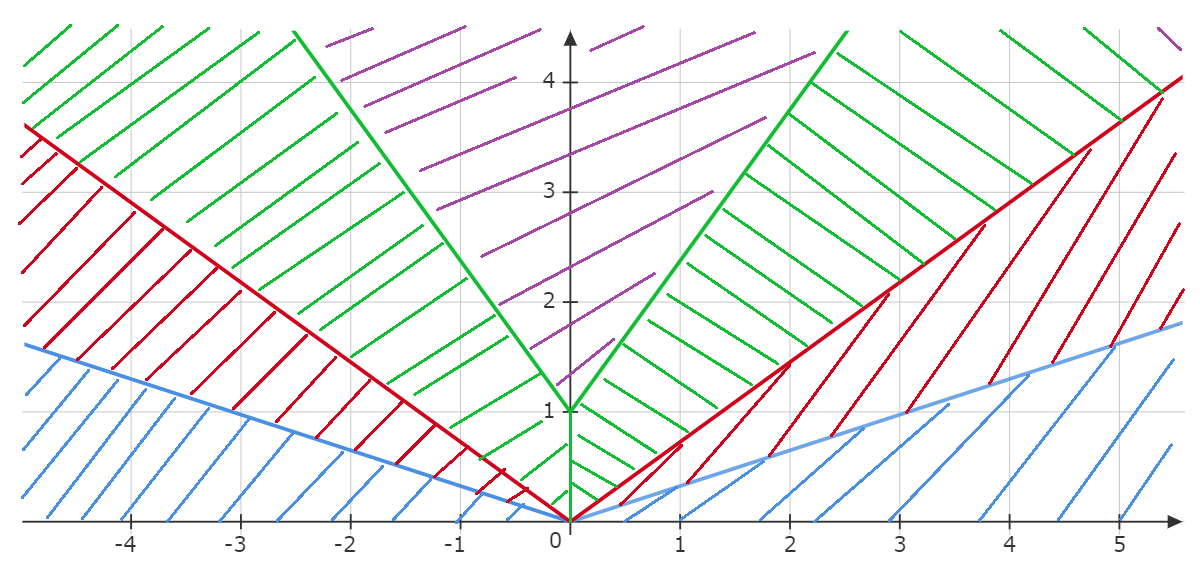
\includegraphics[width=0.5\textwidth]{AlphaFirstDecomposition.png}
	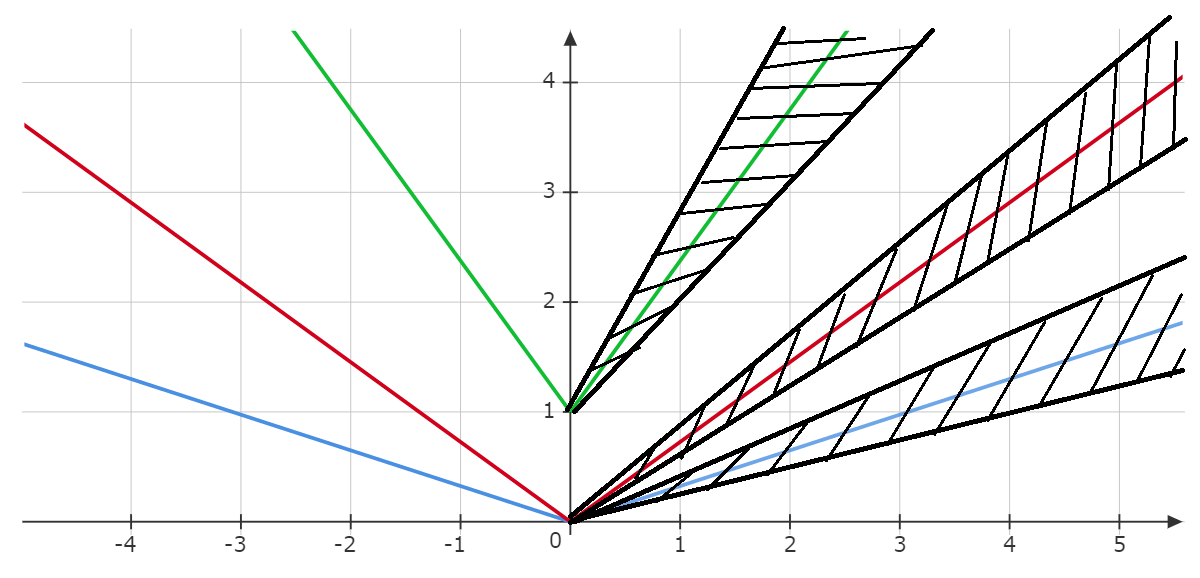
\includegraphics[width=0.5\textwidth]{AlphaSecondDecomposition.png}
	\caption{This figure shows the support of the different automorphisms present in the decomposition of an SQ$_1$-automorphism acting on the upper half plane.}
	\label{fig:SetupSQAut}
\end{figure}
As a remark, notice that this definition is not exactly identical to de definition given in \cite{Ogata2d} due to the translation operators.
\begin{definition}
	Take $\alpha\in\Aut{\AA}$. We say that $\alpha\in\textrm{HAut}_1(\AA)$ if and only if for any $0<\theta<\pi/2$ there exists an $a\in\AA$ and some $\alpha_\sigma\in\Aut{\AA_{C_\theta}\cap\AA_\sigma}$ for each $\sigma\in\{L,R\}$ such that
	\begin{equation}
	\alpha=\Ad{a}\circ\alpha_L\otimes\alpha_R.
	\end{equation}
\end{definition}
We will need one additional class of automorphisms:
\begin{definition}
	Take $\alpha\in\Aut{\AA}$. We say that $\alpha\in\textrm{VAut}_1(\AA)$ if and only if there exists some $a\in\AA$, $\alpha_U\in\Aut{\tau(\AA_{C_\theta^c}\cap\AA_{U})}$ and an $\alpha_D\in\Aut{\tau^{-1}(\AA_{C_\theta^c}\cap\AA_{D})}$ such that
	\begin{equation}
	\alpha=\Ad{a}\circ\alpha_U\otimes\alpha_D.
	\end{equation}
	If furthermore $\alpha_U\circ\beta_g^U=\beta_g^U\circ\alpha_U$ we say that $\alpha\in\textrm{GVAut}_1(\AA)$.
\end{definition}
Now we will state some properties of locally generated automorphisms:
\begin{lemma}\label{lem:PropertiesLocallyGeneratedAutomorphisms}
	Take $H$ an interaction such that there exists a $0<\phi<1$ satisfying that $\norm{H}_{f_\phi}\leq 1$. The following statements now hold (for any $s,t\in\RR$):
	\begin{enumerate}
		\item $\gamma^H_{s;t}\circ\gamma^{H_D}_{t;s}\otimes\gamma^{H_U}_{t;s}\in\textrm{HAut}_1(\AA)$.
		\item $\gamma^H_{s;t}\circ\gamma^{H_L}_{t;s}\otimes\gamma^{H_R}_{t;s}\in\textrm{VAut}_1(\AA)$. If additionally $H$ is a $G$-invariant interaction we even have $\gamma^H_{s;t}\circ\gamma^{H_L}_{t;s}\otimes\gamma^{H_R}_{t;s}\in\textrm{GVQAut}_1(\AA)$.
		\item $\gamma^{H_U}_{s;t}\otimes\gamma^{H_D}_{s;t}\in\textrm{SQAut}_1(\AA)$. If additionally $H$ is a $G$-invariant interaction we even have $\gamma^{H_U}_{s;t}\otimes\gamma^{H_D}_{s;t}\in\textrm{GSQAut}_1(\AA)$.
		\item If $H$ is $G$-invariant then $\gamma^{H}_{t;s}\circ\beta_g^U\circ\gamma^{H}_{s;t}\circ(\beta_g^U)^{-1}\in\textrm{HAut}_1(\AA)$.
		\item $\gamma^{H}_{t;s}\in\textrm{SQAut}_1(\AA)$.
	\end{enumerate}
\end{lemma}
\begin{proof}
	Part 1 is done in Proposition 5.5 in \cite{Ogata2d} and part 4 follows trivially from Part 1. Except for the translation operators in my definition of the $\textrm{SQAut}(\AA)$, part 3 follows from Theorem 5.2 in \cite{Ogata2d}. To show part 3 we therefore have to show that Theorem 5.2 in \cite{Ogata2d} still holds if we replace $\mathcal{C}_0$ and $\mathcal{C}_1$ in the proof by
	\begin{align}
	\mathcal{C}_0&\defeq \left\{C_{[0,\theta_1],\sigma},C_{]\theta_1,\theta_2],\sigma,\rho},C_{]\theta_2,\theta_3],\sigma,\rho}\cup\tau^{\rho}(C_{]\theta_2,\theta_3],\sigma,\rho}),\tau^\rho(C_{]\theta_3,\pi/2],\rho})|\sigma=\{L,R\},\rho=\{U,D\}\right\}\\
	\mathcal{C}_1&\defeq\{C_{[\theta_{0.8},\theta_{1.2}]\cap\sigma\cap\tau},C_{[\theta_{1.8},\theta_{2.2}]\cap\sigma\cap\tau},\tau^\rho(C_{[\theta_{2.8},\theta_{3.2}]\cap\sigma\cap\rho})|\sigma=\{L,R\},\rho=\{U,D\}\}.
	\end{align}
	Take the $\Psi$ from this proof to be our $H$, take $\Psi^{(0)}$ to be $\sum_{C\in\mathcal{C}_0}H_{C}$ (with our new definition of $\mathcal{C}_0$) and take $\Psi^{(1)}\defeq \Psi-\Psi^{(0)}$. Now define $\Xi^{(s)}(Z,t)$ through
	\begin{equation}\label{eq:PropertiesLocallyGeneratedAutomorphismsProofDefinitionXi}
	\Xi^{(s)}(Z,t)\defeq\sum_{m=0}^\infty \sum_{\substack{X\subset Z,\\X(m)=Z}}\Delta_{X(m)}(\gamma^\Psi_{s;t}(\Psi^{(1)}(X;t)))
	\end{equation}
	with these new definitions of $\Psi^{(0)}$ and $\Psi^{(1)}$. We now want so show that for every $t$,
	\begin{equation}
	\sum_{Z\subset\ZZ^2}\left(\Xi^{(s)}(Z,t)-\sum_{C\in\mathcal{C}_1}\id_{Z\subset C}\Xi^{(s)}(Z,t)\right)
	\end{equation}
	is bounded. Following the arguments in equation (5.22) to (5.24) in \cite{Ogata2d} we still get that
	\begin{equation}
	\sum_{\substack{Z\subset\ZZ^2,\\\nexists C\in\mathcal{C}_1:Z\subset C}}\sup_{t\in[0,1]}\norm{\Xi^{(1)}(Z,t)}\leq \frac{8}{C_F}(e^{2I_F(\Psi)}-1)\sum_{\substack{C_1,C_2\in\mathcal{C}_0,\\ C_1\neq C_2}}M(C_1,C_2)
	\end{equation}
	where
	\begin{equation}
	M(C_1,C_2)\defeq \sum_{m\geq 0}\sum_{\substack{X:\\\forall C\in\mathcal{C}_1,X\cap((C^c)(m))\neq\emptyset,\\X\cap C_1\neq\emptyset,X\cap C_2\neq\emptyset}}\left(\sup_{t\in[0,1]}(\norm{\Psi^{(1)}(X;t)})\abs{X}G_F(m)\right)
	\end{equation}
	is now defined using the new $\mathcal{C}_1$. To bound these $M(C_1,C_2)$ we will (just like in \cite{Ogata2d}) differentiate between two cases. That is, the case where $C_1$ and $C_2$ are adjacent\footnote{We say that $C_1$ and $C_2$ are adjacent if and only if $\#(C_1(1)\cap C_2(1))=\infty$.} and the case where they are not. We begin with the latter. In this case we still have in complete analogy with the proof in \cite{Ogata2d} that
	\begin{align}
	M(C_1,C_2)\leq b_0(C_1,C_2) &\defeq \sum_{m\geq 0}\sum_{\substack{X:X\cap C_1\neq\emptyset,\\X\cap C_2\neq\emptyset}}\left(\sup_{t\in[0,1]}(\norm{\Psi^{(1)}(X;t)})\abs{X}G_F(m)\right)\\
	&\leq \norm{\Psi_1}_F\sum_{\substack{x\in C_1\\y\in C_2}}F(d(x,y))\sum_{m=0}^\infty G_F(m)<\infty.
	\end{align}
	\footnote{Here $\Psi_1$ is defined through $\Psi_1(X)=\abs{X}^1 \Psi(X)$.} What is now left to show is the case where $C_1$ and $C_2$ are adjacent. Take $\tilde{C}\in\mathcal{C}_1$ such that $C_1\cap\tilde{C}\neq\emptyset$ and $C_2\cap\tilde{C}\neq\emptyset$. Take $L_1=\partial\tilde{C}/C_2$\footnote{Here $\partial \tilde{C}$ means the boundary of $\tilde C$.} and $L_2=\partial\tilde{C}/C_1$. By following the same reasoning that led to equation (5.36) in \cite{Ogata2d} we get that
	\begin{align}
	M(C_1,C_2)\leq b_0(C_1,C_2/\tilde{C})+b_0(C_1/\tilde{C},C_2)+b_0(\tilde{C}\cap C_2,(C_1\cup C_2)^c)+b_1(C_1\cap\tilde{C},C_2\cap\tilde{C},L_1,L_2)
	\end{align}
	where
	\begin{align}
	b_1(C_1\cap\tilde{C},C_2\cap\tilde{C},L_1,L_2)&\defeq\sum_{m=0}^\infty \sum_{\substack{X\subset \tilde{C}:\\ X\cap C_1\cap\tilde{C}\neq\emptyset\\X\cap C_2\cap\tilde{C}\neq\emptyset\\ X\cap (\tilde{C}^c(m))\neq\emptyset}}\sup_{t\in[0,1]}\norm{\Psi(X;t)}\abs{X}G_F(m)\\
	&\leq \norm{\Psi_1}_F\sum_{m=0}^{\infty}G_F(m)\left(\sum_{\substack{x\in C_2\cap\tilde{C},\\y\in L_1(m)}}+\sum_{\substack{x\in C_1\cap\tilde{C},\\y\in L_2(m)}}\right)F(d(x,y))<\infty.
	\end{align}
	Since the remainder of the proof can remain unchanged from \cite{Ogata2d}, this concludes the proof of item 3. The proof of item 5 just follows from the fact that for any $\alpha_1\in\textrm{SQAut}(\AA)$ and for any $\alpha_2\in\textrm{HAut}(\AA)$ we have that $\alpha_2\circ\alpha_1\in\textrm{SQAut}(\AA)$. We now only need to comment on item 2. We must show that
	\begin{equation}
	(\gamma^H_{s;t}\circ\gamma^{H_L}_{t;s}\otimes\gamma^{H_R}_{t;s})^{-1}=\gamma^{H_L}_{s;t}\otimes\gamma^{H_R}_{s;t}\circ\gamma^H_{t;s}\in\textrm{GVAut}(\AA).
	\end{equation}
	The proof of this starts analogously to the proof of item 1 and 3. We take $\Psi=H$, $\Psi^{(0)}=H_{\tau(C_\theta^c\cap U)}+H_{\tau^{-1}(C_\theta^c\cap D)}$ and $\Psi^{(1)}=\Psi-\Psi^{(0)}$. Define $\Xi^{(s)}(Z;t)$ again through equation \eqref{eq:PropertiesLocallyGeneratedAutomorphismsProofDefinitionXi}. In analogy to what was done in equation (5.54) in \cite{Ogata2d} we obtain
	\begin{equation}
	\sum_{\substack{Z:Z\nsubseteq \tau(C_\theta^c\cap U)\\\text{and }Z\nsubseteq \tau^{-1}(C_\theta^c\cap D)}}\sup_{t\in[0,1]}\norm{\Xi^{(1)}(Z,t)}\leq \frac{8}{C_F}(e^{2I_F(\Psi)}-1)\sum_{m=0}^\infty\sum_{\substack{X:X(m)\nsubseteq \tau(C_\theta^c\cap U)\\\text{and }X(m)\nsubseteq \tau^{-1}(C_\theta^c\cap D)}} \sup_{t\in[0,1]}\norm{\Psi^{(1)}(X;t)}\abs{X}G_F(m).
	\end{equation}
	If $X$ in the last line has a non-zero contribution, then at least one of the following occurs:
	\begin{enumerate}
		\item $X\cap (W(C_\theta)\cap L)\neq\emptyset$ and $X\cap R\neq\emptyset$.
		\item $X\cap (W(C_\theta)\cap R)\neq\emptyset$ and $X\cap L\neq\emptyset$.
		\item $X\subset W(C_\theta)^c$ and
		\begin{enumerate}
			\item $X\subset U,X\subset D$, or
			\item $X\subset U,X\subset L,X\subset R$ and $X(m)\cap (\tau^{-1}(C_\theta^c\cap D))^c\neq \emptyset$, or
			\item $X\subset D,X\subset L,X\subset R$ and $X(m)\cap (\tau(C_\theta^c\cap U))^c\neq \emptyset$.
		\end{enumerate}
	\end{enumerate}
	This shows that we have a bound
	\begin{align}
	&\sum_{\substack{Z:Z\nsubseteq \tau(C_\theta^c\cap U)\\\text{and }Z\nsubseteq \tau^{-1}(C_\theta^c\cap D)}}\sup_{t\in[0,1]}\norm{\Xi^{(1)}(Z,t)}\\
	\nonumber
	&\leq \frac{8}{C_F}(e^{2I_F(\Psi)}-1)(b_0(W(C_\theta)\cap L,R)+b_0(L,W(C_\theta)\cap R)+b_0(W(C_\theta)^c\cap U,W(C_\theta)^c\cap D)\\
	\nonumber
	&\qquad+b_1(W(C_\theta)^c\cap U\cap L,W(C_\theta)^c\cap U\cap L,L\cap\partial(W(C_\theta)^c\cap U),R\cap\partial(W(C_\theta)^c\cap U))\\
	&\qquad b_1(W(C_\theta)^c\cap D\cap L,W(C_\theta)^c\cap D\cap R,L\cap\partial(W(C_\theta)^c\cap D),R\cap\partial(W(C_\theta)^c\cap D)))<\infty.
	\end{align}
	This concludes the proof.
\end{proof}
This implies certain things for our locally generated automorphisms.
From these four statements we can prove the following results:
\begin{lemma}\label{lem:TwoAngleLemmaPart1}
	Take $H$ an interaction such that there exists a $0<\phi<1$ satisfying that $\norm{H}_{f_\phi}\leq 1$. Take $\theta_1$ and $\theta_2$ such that $0<\theta_1<\theta_2<\pi/2$ then for all $\Theta\in\Aut{\AA_{W(C_{\theta_2})^c}}$ and $s,t\in\RR$ there exists an $a_1\in\UU(\AA)$ and a $\tilde{\Theta}\in \Aut{\AA_{W(C_{\theta_1})^c}}$ such that
	\begin{equation}\label{eq:TwoAngleLemmaPart1Equation1}
	\gamma^{H}_{t;s}\circ\Theta\circ\gamma^{H}_{s;t}=\Ad{a_1}\circ\tilde{\Theta}.
	\end{equation}
\end{lemma}
\begin{proof}
	We have that
	\begin{equation}
	\gamma^{H}_{t;s}\circ\Theta\circ\gamma^{H}_{s;t}=\gamma^{H_D}_{t;s}\otimes\gamma^{H_U}_{t;s}\circ\gamma^{H_D}_{s;t}\otimes\gamma^{H_U}_{s;t}\circ\gamma^{H}_{t;s}\circ\Theta\circ\gamma^{H}_{s;t}\circ\gamma^{H_D}_{t;s}\otimes\gamma^{H_U}_{t;s}\circ\gamma^{H_D}_{s;t}\otimes\gamma^{H_U}_{s;t}.
	\end{equation}
	Using that $\gamma^{H}_{s;t}\circ\gamma^{H_D}_{t;s}\otimes\gamma^{H_U}_{t;s}\in\textrm{HAut}_1(\AA)$ we get that there exists some $a\in\AA$ and $\eta\in\Aut{\AA_{C_\theta}}$ such that
	\begin{align}
	\gamma^{H}_{t;s}\circ\Theta\circ\gamma^{H}_{s;t}&=\Ad{a}\circ \gamma^{H_D}_{t;s}\otimes\gamma^{H_U}_{t;s}\circ\eta_{s;t}^{-1}\circ\Theta\circ\eta_{s;t}\circ\gamma^{H_D}_{s;t}\otimes\gamma^{H_U}_{s;t}\\
	&=\Ad{a}\circ \gamma^{H_D}_{t;s}\otimes\gamma^{H_U}_{t;s}\circ\Theta\circ\gamma^{H_D}_{s;t}\otimes\gamma^{H_U}_{s;t}.
	\end{align}
	Since by \ref{lem:PropertiesLocallyGeneratedAutomorphisms} part 3 $\gamma^{H_D}_{s;t}\otimes\gamma^{H_U}_{s;t}\in\textrm{GSQAut}_1(\AA)$ the result follows.
\end{proof}
\begin{lemma}\label{lem:TwoAngleLemmaPart2}
	Take $H$ an interaction such that there exists a $0<\phi<1$ satisfying that $\norm{H}_{f_\phi}\leq 1$. Take $\theta_1$ and $\theta_2$ such that $0<\theta_1<\theta_2<\pi/2$. Then for all $\eta_{g}^{\sigma}\in\Aut{\AA_{C_{\theta_1}}\cap\AA_{\sigma}}$ (where $\sigma\in\{L,R\}$ and $g\in G$) and $s,t\in\RR$ there exist $a_{2},\in\UU(\AA),a_{3,\sigma}\in\UU(\AA_\sigma)$ and some $\tilde{\eta}_{\sigma}^g\in \Aut{\AA_{C_{\theta_2}}\cap\AA_{\sigma}}$ such that
	\begin{align}
	\label{eq:TwoAngleLemmaPart2Equation1}
	\gamma^{H}_{t;s}\circ\eta_{g}^L\otimes\eta_{g}^R\circ\gamma^{H}_{s;t}&=\Ad{a_2}\circ(\tilde\eta_{g}^L \otimes\tilde\eta_{g}^R)\\
	\label{eq:TwoAngleLemmaPart2Equation2}
	\gamma^{H_\sigma}_{t;s}\circ\eta_g^\sigma\circ\gamma^{H_\sigma}_{s;t}&=\Ad{a_{3,\sigma}}\circ \tilde\eta_{g}^\sigma.
	\end{align}
\end{lemma}
\begin{proof}
	In this proof, take $\Hsplit=H_L+H_R$. First we show that equation \eqref{eq:TwoAngleLemmaPart2Equation2} implies equation \eqref{eq:TwoAngleLemmaPart2Equation1}. This is because using equation \eqref{eq:TwoAngleLemmaPart2Equation1} we get that
	\begin{align}
	\gamma^H_{t;s}\circ\eta_g\circ\gamma^{H}_{s;t}&=\gamma^H_{t;s}\circ\gamma^{\Hsplit}_{s;t}\circ\gamma^{\Hsplit}_{t;s}\circ\eta_g\circ\gamma^{\Hsplit}_{s;t}\circ\gamma^{\Hsplit}_{t;s}\circ\gamma^H_{s;t}\\
	&=\gamma^H_{t;s}\circ\gamma^{\Hsplit}_{s;t}\circ\Ad{a_{3,L}\otimes a_{3,R}}\circ\tilde{\eta}_g\circ\gamma^{\Hsplit}_{t;s}\circ\gamma^H_{s;t}.
	\end{align}
	If one now uses the fact that $\gamma^H_{t;s}\circ\gamma^{\Hsplit}_{s;t}\in\textrm{GVAut}_1(\AA)$ (see lemma \ref{lem:PropertiesLocallyGeneratedAutomorphisms} item 2) the implication follows. To finish the proof we now only have to use the fact that the $\gamma^{H_\sigma}_{0;1}$ are in $\textrm{SQAut}_1(\AA_\sigma)$.
\end{proof}
Additionally when we add the group action, we get:
\begin{lemma}\label{lem:TwoAngleLemmaPart3}
	Take $H$ a $G$-invariant interaction such that there exists a $0<\phi<1$ satisfying that $\norm{H}_{f_\phi}\leq 1$. Take $\theta_1$ and $\theta_2$ such that $0<\theta_1<\theta_2<\pi/2$. Then for all $\eta_{g}^{\sigma}\in\Aut{\AA_{C_{\theta_1}}\cap\AA_{\sigma}}$ (where $\sigma\in\{L,R\}$ and $g\in G$) and $s,t\in\RR$ there exist $a_{2},\in\UU(\AA),a_{3,\sigma}\in\UU(\AA_\sigma)$ and some $\tilde{\eta}_{\sigma}^g\in \Aut{\AA_{C_{\theta_2}}\cap\AA_{\sigma}}$ such that
	\begin{align}
	\label{eq:TwoAngleLemmaPart3Equation1}
	\gamma^{H}_{t;s}\circ\eta_{g}^L\otimes\eta_{g}^R\circ\beta_g^U\circ\gamma^{H}_{s;t}&=\Ad{a_2}\circ(\tilde\eta_{g}^L \otimes\tilde\eta_{g}^R)\circ\beta_g^U\\
	\label{eq:TwoAngleLemmaPart3Equation2}
	\gamma^{H_\sigma}_{t;s}\circ\eta_g^\sigma\circ\beta_g^{\sigma U}\circ\gamma^{H_\sigma}_{s;t}&=\Ad{a_{3,\sigma}}\circ \tilde\eta_{g}^\sigma\circ\beta_g^{\sigma U}.
	\end{align}
\end{lemma}
\begin{proof}
	In this proof, take again $\Hsplit=H_L+H_R$. First we show that equation \eqref{eq:TwoAngleLemmaPart3Equation2} implies equation \eqref{eq:TwoAngleLemmaPart3Equation1}. This is because using (the inverse of) equation \eqref{eq:TwoAngleLemmaPart3Equation1} we get that
	\begin{align}
	&\gamma^H_{t;s}\circ\eta_g\circ\beta_g^U\circ\gamma^H_{s;t}\circ\beta_{g^{-1}}^U\circ(\tilde{\eta}_g)^{-1}\\
	&=(\text{Inner})\circ \gamma^H_{t;s}\circ\eta_g\circ\beta_g^U\circ\gamma^H_{s;t}\circ\gamma^\Hsplit_{t;s}\circ\beta_{g^{-1}}^U\circ(\eta_g)^{-1}\circ\gamma^\Hsplit_{s;t}\circ\underline{\gamma^H_{t;s}\circ\gamma^H_{s;t}}.
	\end{align}
	Now using the fact that by lemma \ref{lem:PropertiesLocallyGeneratedAutomorphisms} item 2, $\gamma^H_{s;t}\circ\gamma^\Hsplit_{t;s}\in\textrm{GVAut}_1(\AA)$ this gives us
	\begin{align}
	&=(\text{Inner})\circ\stkout{\gamma^H_{t;s}\circ\eta_g\circ\beta_g^U\circ\beta_{g^{-1}}^U\circ(\eta_g)^{-1}\circ\gamma^H_{s;t}}.
	\end{align}
	By taking $a_2$ such that $\Ad{a_2}$ is this inner automorphism, we can conclude the proof that equation \eqref{eq:TwoAngleLemmaPart3Equation2} implies equation \eqref{eq:TwoAngleLemmaPart3Equation1}. Now we only have to prove equation \eqref{eq:TwoAngleLemmaPart3Equation2}. To finish the proof we now only have to use the fact that the $\gamma^{H_\sigma}_{0;1}$ are in $\textrm{GSQAut}_1(\AA_\sigma)$.
\end{proof}
\subsection{The two translation symmetries}
This section will define the classes of automorphisms required in the assumptions and proofs about the $H^1$-valued translation index. In analogy with section 2.1 from \cite{Ogata2d} we will define some classes of automorphisms (see figure \ref{fig:SetupSQAut2}):
\begin{definition}\label{def:SQAut2}
	Take $\alpha\in\Aut{\AA}$. We say that $\alpha\in\textrm{SQAut}_2(\AA)$ if and only if for any $0<\theta_{0.8}<\theta_{1}<\theta_{1.2}<\theta_{1.8}<\theta_{2}<\theta_{2.2}<\theta_{2.8}<\theta_3<\theta_{3.2}<\pi/2$ there exist $a\in\AA$, $\alpha_{[0,\theta_1], \sigma}\in\Aut{\AA_{\nu^{\sigma}(C_{[0,\theta_1]}\cap\sigma)}},\:\alpha_{]\theta_1,\theta_2],\sigma,\rho}\in\Aut{\AA_{\nu^{\sigma}(C_{]\theta_1,\theta_2]}\cap\rho\cap\sigma)}},\:\alpha_{]\theta_2,\theta_3],\sigma,\rho}\in\Aut{\AA_{(W(C_{[0,\theta_3]})/\nu^\sigma(C_{[0,\theta_2]}\cap\sigma))\cap\rho\cap\sigma)}},\\
	\alpha_{]\theta_3,\pi/2],\rho}\in\Aut{\AA_{\tau^\rho(C_{[\theta_3,\pi/2]}\cap\rho)}},\:\alpha_{]\theta_{0.8},\theta_{1.2}],\sigma,\rho}\in\Aut{\AA_{\nu^{\sigma}(C_{]\theta_{0.8},\theta_{1.2}]}\cap\rho\cap\sigma)}},\\
	\alpha_{]\theta_{1.8},\theta_{2.2}],\sigma,\rho}\in\Aut{\AA_{\nu^{\sigma}(C_{]\theta_{1.8},\theta_{2.2}]}\cap\rho\cap\sigma)}}$ and  $\alpha_{]\theta_{2.8},\theta_{3.2}],\sigma,\rho}\in\Aut{\AA_{\tau^{\rho}(C_{]\theta_{2.8},\theta_{3.2}]}\cap\rho\cap\sigma)}}$ for any $\rho\in\{U,D\}$ and $\sigma\in\{L,R\}$ (here $\tau^U=\tau$, $\tau^D=\tau^{-1}$, $\nu^R=\nu$ and $\nu^L=\nu^{-1}$) such that
	\begin{equation}
	\alpha=\Ad{a}\circ \bigotimes_{\sigma}\alpha_{[0,\theta_1],\sigma}\circ\bigotimes_{\sigma,\rho}\alpha_{]\theta_1,\theta_2],\sigma,\rho}\circ\bigotimes_{\rho}\alpha_{[\theta_3,\pi/2]}\circ\bigotimes_{\rho,\sigma}\left(\alpha_{]\theta_{0.8},\theta_{1.2}],\rho,\sigma}\otimes\alpha_{]\theta_{1.8},\theta_{2.2}],\rho,\sigma}\otimes\alpha_{]\theta_{2.8},\theta_{3.2}],\rho,\sigma} \right).
	\end{equation}
	If additionally everything (except $a$) commutes with $\beta_g^U$ we say that $\alpha\in \textrm{GSQAut}_2(\AA)$.
\end{definition}
\begin{figure}
	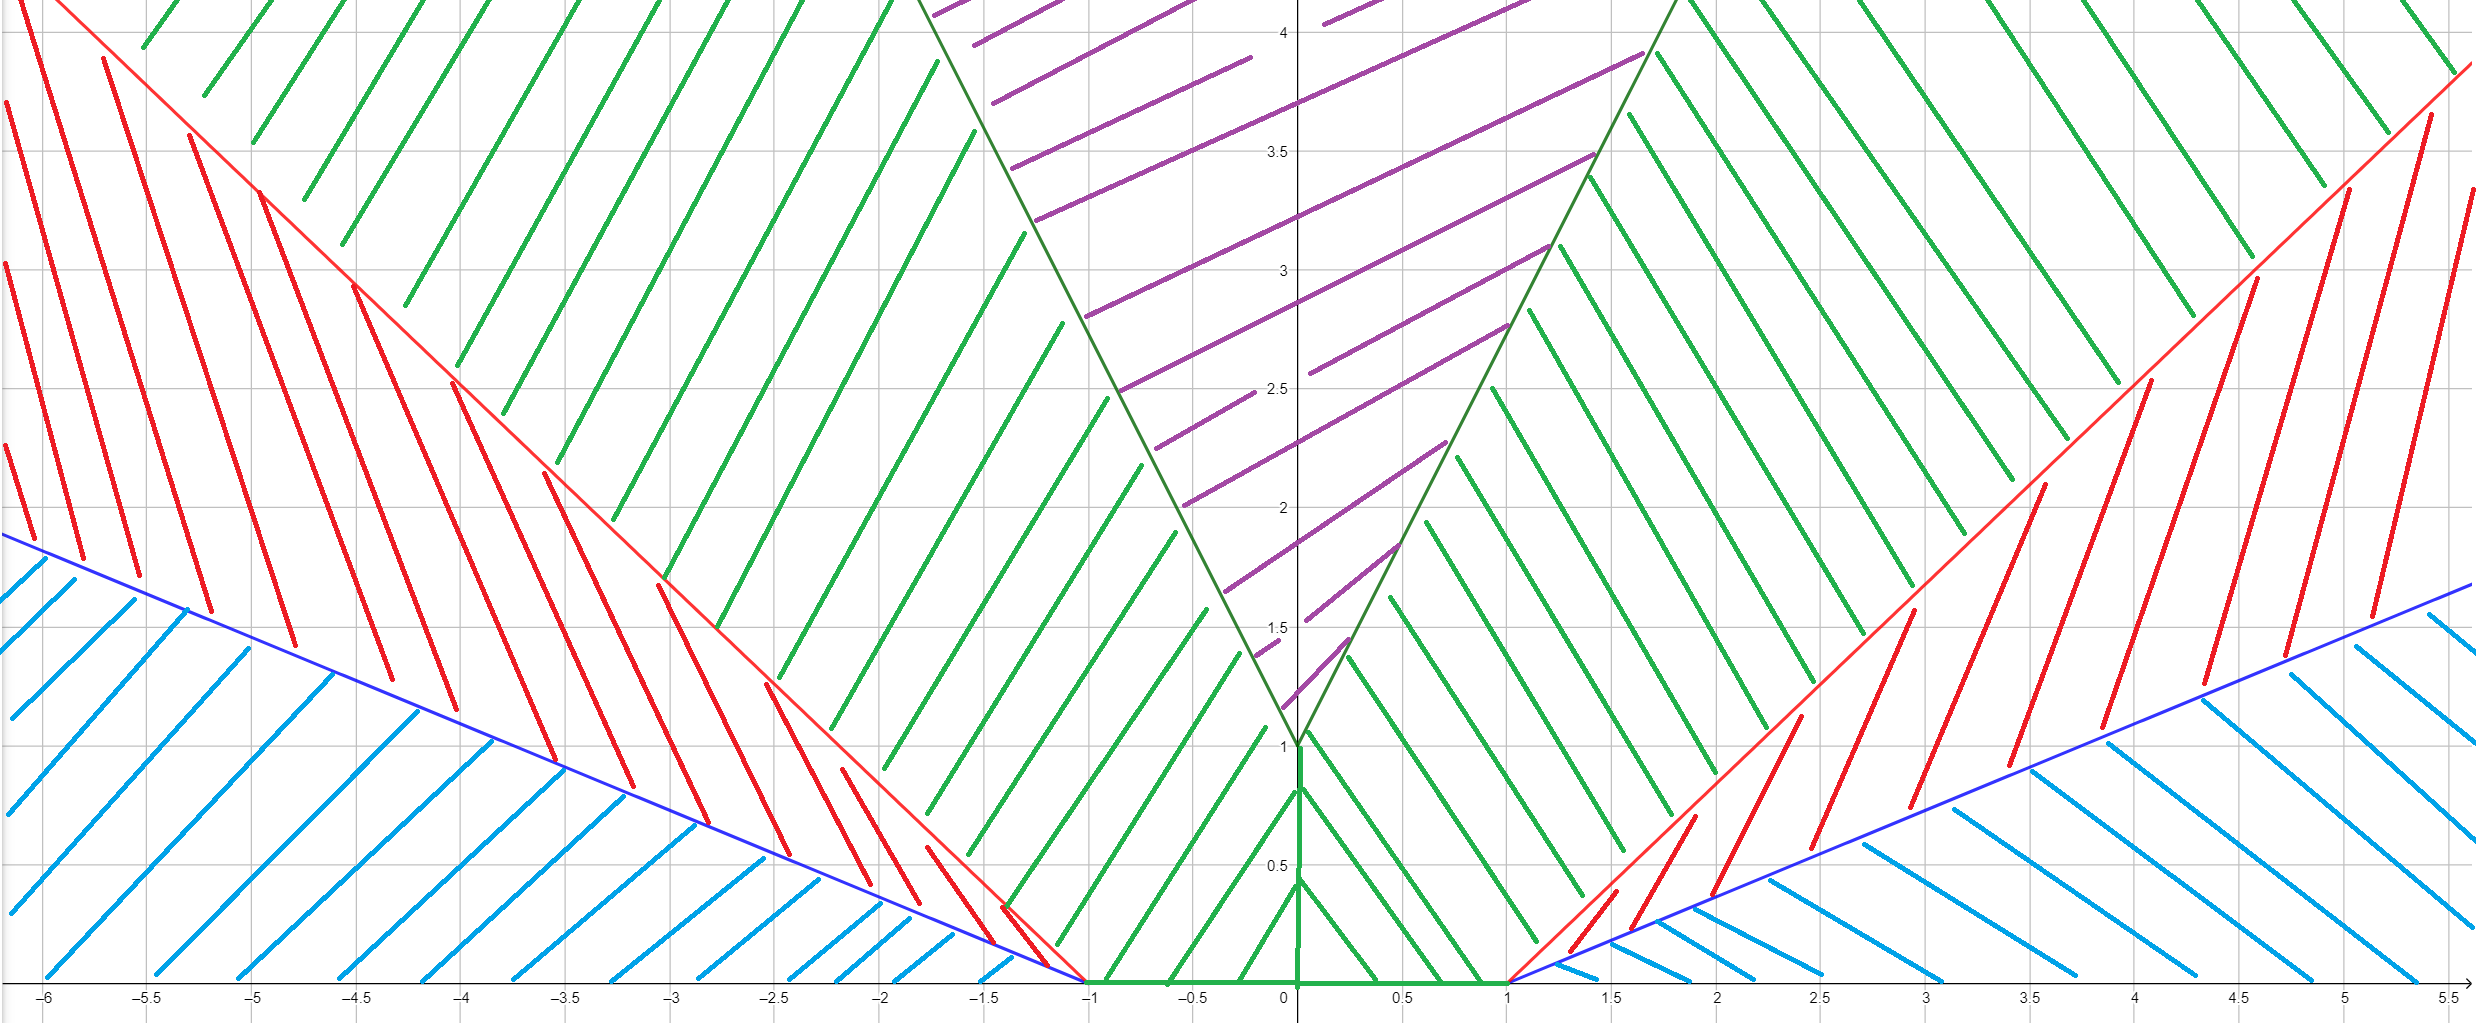
\includegraphics[width=0.5\textwidth]{AlphaFirstDecomposition2.png}
	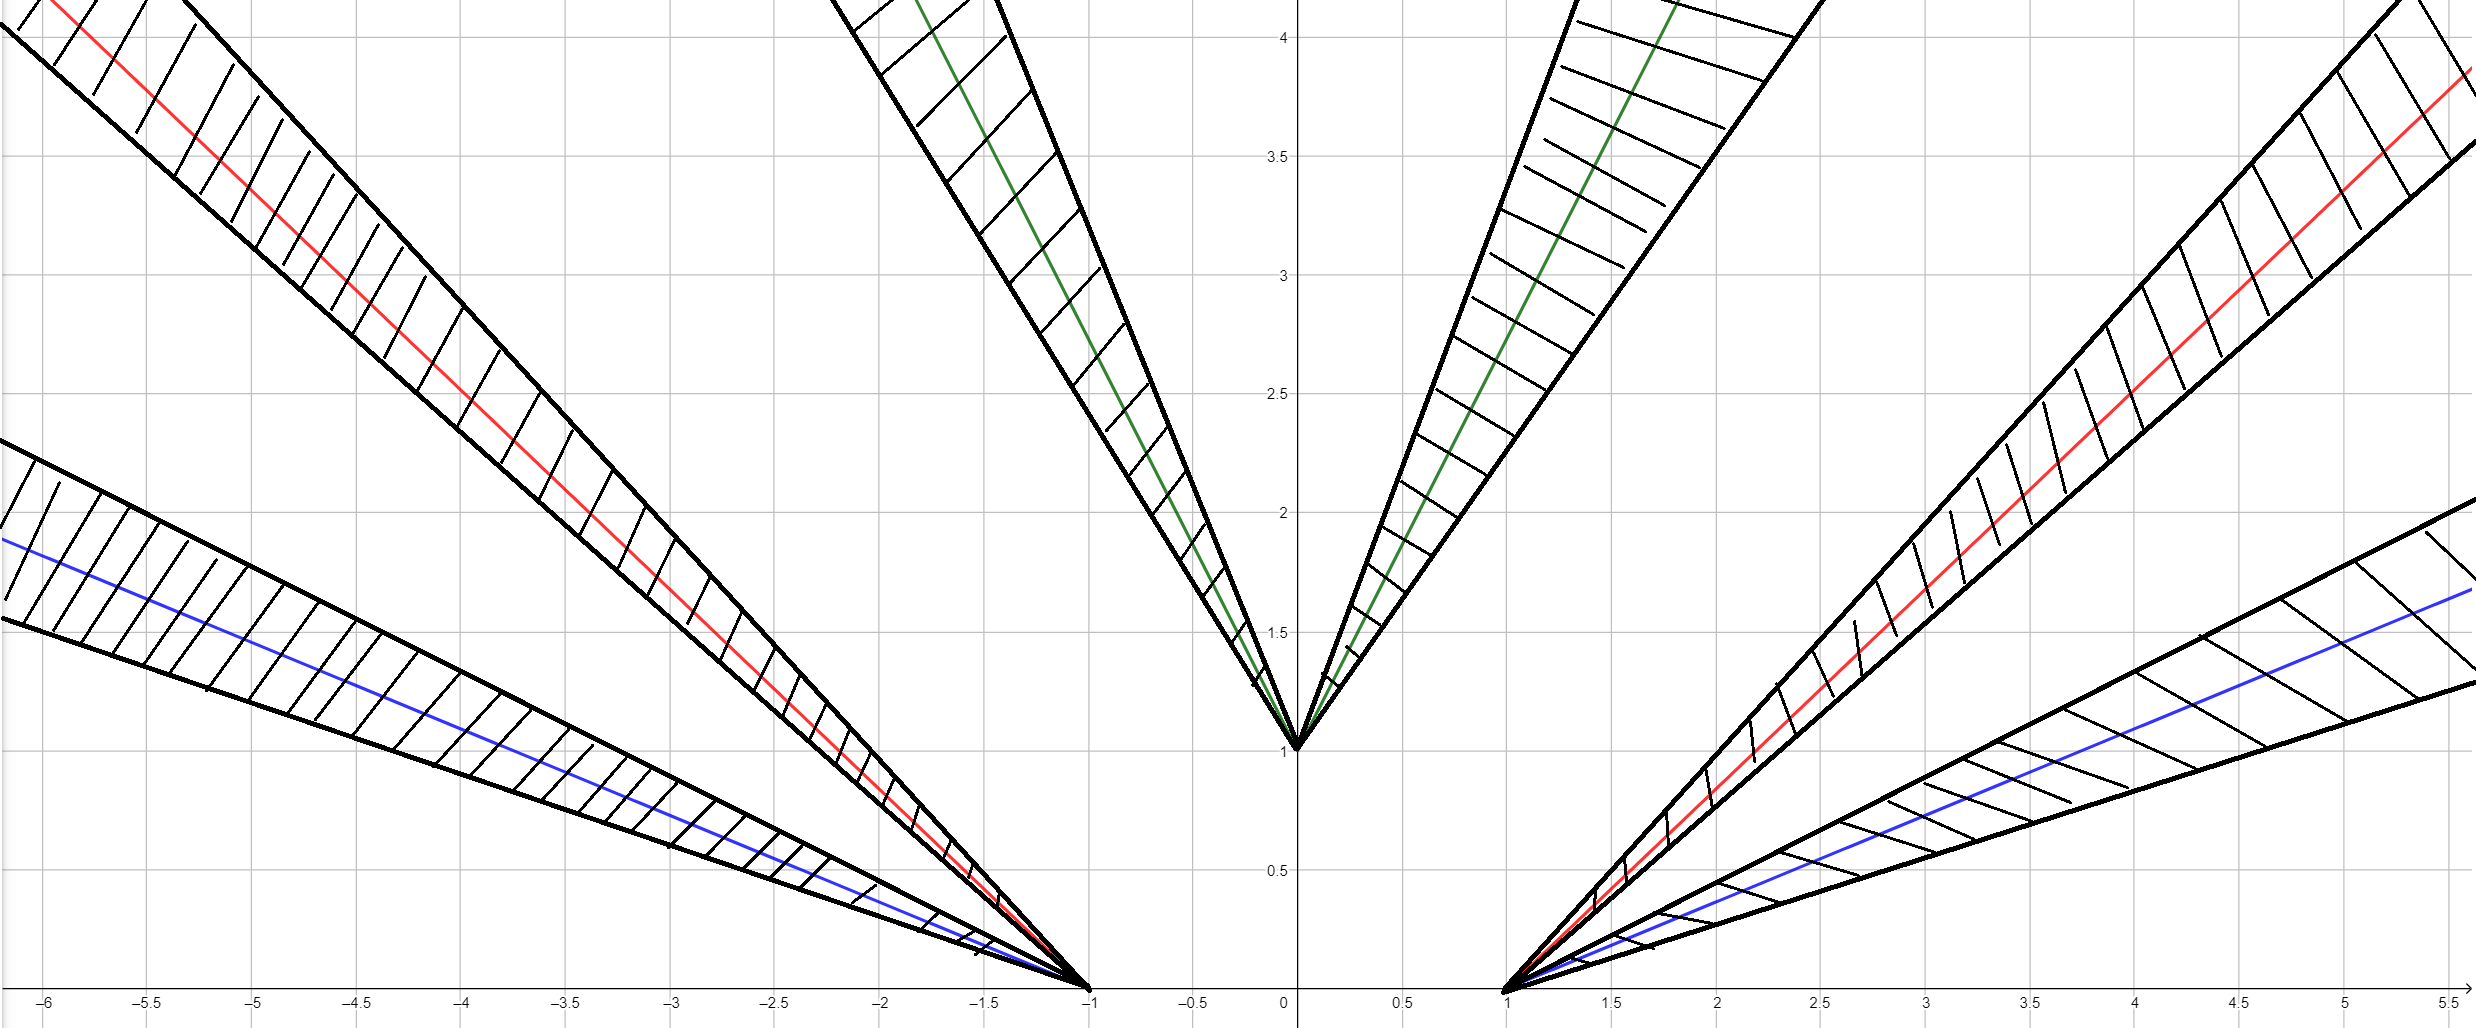
\includegraphics[width=0.5\textwidth]{AlphaSecondDecomposition2.png}
	\caption{This figure shows the support of the different automorphisms present in the decomposition of an SQ$_2$-automorphism acting on the upper half plane.}
	\label{fig:SetupSQAut2}
\end{figure}
We now have to define a different horizontal automorphism:
\begin{definition}
	Take $\alpha\in\Aut{\AA}$. We say that $\alpha\in\textrm{HAut}_2(\AA)$ if and only if for any $0<\theta<\pi/2$ there exists an $a\in\AA$ and some $\alpha_\sigma\in\Aut{\AA_{\nu^{\sigma}(C_\theta\cap\sigma)}}$ for each $\sigma\in\{L,R\}$ such that
	\begin{equation}
	\alpha=\Ad{a}\circ\alpha_L\otimes\alpha_R.
	\end{equation}
\end{definition}
The main reason why we introduce this new class of automorphisms is that if $\alpha\in\textrm{HAut}_2(\AA)$ we automatically have that the translations of $\alpha$ in the horizontal directions, $\nu^{-1}\circ\alpha\circ\nu$ and $\nu\circ\alpha\circ\nu^{-1}$ are elements of $\textrm{HAut}_1(\AA)$. We will let the definition of vertical automorphism stay the same, namely $\textrm{VAut}_2(\AA)=\textrm{VAut}_1(\AA)$ and $\textrm{GVAut}_2(\AA)=\textrm{GVAut}_1(\AA)$.
\begin{lemma}\label{lem:PropertiesLocallyGeneratedAutomorphismsTwoTranslations}
	Lemma \ref{lem:PropertiesLocallyGeneratedAutomorphisms} will still be true when we exchange all the $_1$'s for $_2$'s.
\end{lemma}
\begin{proof}
	Completely equivalent to the proof of \ref{lem:PropertiesLocallyGeneratedAutomorphisms}.
\end{proof}
\begin{lemma}\label{lem:TwoAngleLemmaPart2ForTwoTranlations}
	Take $\theta_1$ and $\theta_2$ such that $0<\theta_1<\theta_2<\pi/2$. Then for all $\eta_{g}^{\sigma}\in\Aut{\AA_{\nu^{\sigma}(C_{\theta_1}\cap\sigma)}}$ (where $\sigma\in\{L,R\}$ and $g\in G$), there exist $a_{2},\in\UU(\AA),a_{3,\sigma}\in\UU(\AA_{\nu^{\sigma}(\sigma)})$ and some $\tilde{\eta}_{\sigma}^g\in \Aut{\AA_{\nu^\sigma(C_{\theta_2}\cap\sigma)}}$ such that
	\begin{align}
	\label{eq:TwoAngleLemmaPart2Equation1ForTwoTranlations}
	\gamma^{H}_{1;0}\circ\eta_{g}^L\otimes\eta_{g}^R\circ\gamma^{H}_{0;1}&=\Ad{a_2}\circ(\tilde\eta_{g}^L \otimes\tilde\eta_{g}^R)\\
	\label{eq:TwoAngleLemmaPart2Equation2ForTwoTranlations}
	\gamma^{H_{\nu^{\sigma}(\sigma)}}_{1;0}\eta_g^\sigma\gamma^{H_{\nu^\sigma(\sigma)}}_{0;1}&=\Ad{a_{3,\sigma}}\circ \tilde\eta_{g}^\sigma.
	\end{align}
\end{lemma}
\begin{proof}
	Analogous to the proof of \ref{lem:TwoAngleLemmaPart2}.
\end{proof}
Additionally when we add the group action, we get:
\begin{lemma}\label{lem:TwoAngleLemmaPart3ForTwoTranlations}
	Take $H$ a $G$-invariant interaction such that there exists a $0<\phi<1$ satisfying that $\norm{H}_{f_\phi}\leq 1$. Take $\theta_1$ and $\theta_2$ such that $0<\theta_1<\theta_2<\pi/2$. Then for all $\eta_{g}^{\sigma}\in\Aut{\AA_{C_{\theta_1}}\cap\AA_{\sigma}}$ (where $\sigma\in\{L,R\}$ and $g\in G$), there exist $a_{2},\in\UU(\AA),a_{3,\sigma}\in\UU(\AA_\sigma)$ and some $\tilde{\eta}_{\sigma}^g\in \Aut{\AA_{\nu^\sigma(C_{\theta_2}\cap\sigma)}}$ such that
	\begin{align}
	\label{eq:TwoAngleLemmaPart3Equation1ForTwoTranlations}
	\gamma^{H}_{1;0}\circ\eta_{g}^L\otimes\eta_{g}^R\circ\beta_g^U\circ\gamma^{H}_{0;1}&=\Ad{a_2}\circ(\tilde\eta_{g}^L \otimes\tilde\eta_{g}^R)\circ\beta_g^U\\
	\label{eq:TwoAngleLemmaPart3Equation2ForTwoTranlations}
	\gamma^{H_\sigma}_{1;0}\circ\eta_g^\sigma\circ\beta_g^{\sigma U}\circ\gamma^{H_\sigma}_{0;1}&=\Ad{a_{3,\sigma}}\circ \tilde\eta_{g}^\sigma\circ\beta_g^{\sigma U}.
	\end{align}
\end{lemma}
\begin{proof}
	Analogous to the proof of \ref{lem:TwoAngleLemmaPart3}.
\end{proof}
In what follows, let $\HsplitTilde\defeq H_{\nu^{-1}(L)}+H_{\nu(R)}$. We will need the following lemma:
\begin{lemma}\label{lem:SplittedAutomorphismAfterTranslatedIsVertical}
	There exist maps
	\begin{align}
	A_L&:[0,1]\rightarrow \UU(\AA_L):\lambda\mapsto A_{L}(\lambda)&A_R&:[0,1]\rightarrow \UU(\AA_R):\lambda\mapsto A_{R}(\lambda)
	\end{align}
	both continuous in norm topology and
	\begin{align}
	\Phi^{\mu\nu}:[0,1]\rightarrow\Aut{\AA_{W(C_\theta)^c\cap\mu\cap\nu}}:\lambda\mapsto \Phi^{\mu\nu}(\lambda)
	\end{align}
	where $\mu\in\{U,D\}$ and $\nu\in\{L,\nu(R)\}$, all four continuous in  strong\footnote{Meaning that $\Phi^{\mu\nu}(\lambda)(A)$ is continuous for all $A\in\AA$.} topology, satisfying that
	\begin{align}
	\nu\circ\gamma^{\HsplitTilde}_{0;\lambda}\circ\nu^{-1}\circ\gamma^{\HsplitTilde}_{\lambda;0}&=\gamma^{H_L}_{0;\lambda}\otimes\gamma^{H_{\nu\circ\nu(R)}}_{0;\lambda}\circ\gamma^{\HsplitTilde}_{\lambda;0}\\
	\label{eq:TranslatingSplittedTimeEvolutionAppendix}
	&=\Ad{A_L(\lambda)}\otimes\Ad{A_R(\lambda)}\circ\bigotimes_{\substack{\mu\in\{U,D\},\\\nu\in\{L,\nu(R)\}}}\Phi^{\mu\nu}(\lambda)
	\end{align}
	and that $\Phi^{\mu\nu}\circ\beta_g=\beta_g\circ\Phi^{\mu\nu}$.
\end{lemma}
\begin{proof}
	The proof of this is very similar to all the other proofs in this section. We will go over the highlights. We want to define an $A_L(\lambda)$ and a $\Phi^{U,L}\otimes\Phi^{D,L}$ satisfying
	\begin{equation}
	\Ad{A_L(\lambda)}\circ\Phi^{U,L}\otimes\Phi^{D,L}(\lambda)=\gamma^{H_L}_{0;\lambda}\circ\gamma^{H_{\nu^{-1}(L)}}_{\lambda;0}
	\end{equation}
	and similarly for the right side. We will only work out this side as the other calculation is analogous. We do this in two steps. First we find an interaction $\Xi$ satisfying
	\begin{equation}
	\gamma^\Xi_{0;\lambda}=\gamma^{H_L}_{0;\lambda}\circ\gamma^{H_{\nu^{-1}(L)}}_{\lambda;0}.
	\end{equation}
	We can do this by taking the usual
	\begin{equation}
	\Xi(Z,t)\defeq \sum_{m=0}^{\infty}\sum_{\substack{X\subset Z\\X(m)=Z}}\Delta_{X(m)}(\gamma^{H_{\nu^{-1}(L)}}_{0;t}(\tilde{H}(X,t)))
	\end{equation}
	where $\tilde{H}\defeq H_L-H_{\nu^{-1}(L)}$. We can now define
	\begin{equation}
	\Phi^{\mu L}(\lambda)\defeq\gamma^{\Xi_{W(C_\theta)^c\cap\mu\cap L}}_{0;\lambda}.
	\end{equation}
	This means that we can satisfy \ref{eq:TranslatingSplittedTimeEvolutionAppendix} if
	\begin{align}
	\Ad{A_L}&=\gamma^{\Xi}_{0;\lambda}\circ\gamma^{\Xi'}_{\lambda;0}&\Xi'&\defeq \Xi_{W(C_\theta)^c\cap U\cap L}+\Xi_{W(C_\theta)^c\cap D\cap L}.
	\end{align}
	Using the same argument as before, this can be realised when we have
	\begin{equation}
	\Ad{A_L(\lambda)}=\gamma^{\tilde\Xi}_{0;\lambda}
	\end{equation}
	where
	\begin{equation}
	\tilde\Xi(Z,t)\defeq \sum_{m=0}^{\infty}\sum_{\substack{X\subset Z\\X(m)=Z}}\Delta_{X(m)}(\gamma^{\Xi'}_{0;t}(\Xi(X,t)-\Xi'(X,t))).
	\end{equation}
	The last part of the proof is to show that $\norm{\sum_{Z\in\mathfrak{B}_{\ZZ^2}}\tilde\Xi(Z,t)}<\infty$ which can be done using similar techniques as before. This means that we can simply define
	\begin{equation}
	A_L(\lambda)\defeq\mathcal{T}\exp(-i\int_0^\lambda \d s\: \sum_{Z\in \mathfrak{B}_{\ZZ^2}}\tilde{\Xi}(Z,s))
	\end{equation}
	and this is by construction bounded and continuous in $\lambda$.
\end{proof}
\section{Operators belonging to $\omega\circ\gamma^H_{0;1}$}
We will complete the proof of theorem \ref{thrm:IndexInvariantUnderLGA}.
\begin{lemma}\label{lem:OperatorsBelongingToOmegaAfterH}
	The following operators now belong to $\omega\circ\gamma^{H}_{0;1}:$
	\begin{align}
	\label{eq:IndexInvariantUnderLGANewOperator1Appendix}
	\tilde{v}&=\pi_0(A_1)v\pi_0(A_1)^\dagger\\
	\label{eq:IndexInvariantUnderLGANewOperator2Appendix}
	\tilde{W}_g&=\pi_0(A_1)\phi_1(\delta^L_g\otimes\delta^R_g)\phi_2( W_g)\pi_0(A_1^\dagger)\\
	\label{eq:IndexInvariantUnderLGANewOperator3Appendix}
	\tilde u_\sigma(g,h)&=\pi_0(A_1) \phi_1\left(\delta^\sigma_g W_g\delta^\sigma_h W_g^\dagger u_\sigma(g,h)(\delta^\sigma_{gh})^\dagger\right)\pi_0(A_1)^\dagger\\
	\label{eq:IndexInvariantUnderLGANewOperator4Appendix}
	\tilde{K}_g^\sigma&=\pi_0(A_1)\phi_1(v^\dagger \delta_g^\sigma v K_g^\sigma (\delta_g^\sigma)^\dagger) \pi_0(A_1)^\dagger
	\end{align}
	where $\delta^\sigma_g=\pi_0\circ\alpha_0\circ\Theta\circ\gamma^{H_\sigma}_{0;1}(A^\sigma_{2,g})$ with $A^\sigma_{2,g}$ defined in \ref{eq:IndexInvariantUnderLGAEtaTildeDefiniton2} and $A_1$ was defined in equation \eqref{eq:ProofThatTheH2IndexIsInvariantUnderLGA's_Definition_A1}.
\end{lemma}
\begin{proof}
	To do this we first state that a small calculation shows that $\forall x\in\UU(\HH_0)$ satisfying that $\exists\xi\in\Aut{\AA}$ such that
	\begin{equation}
	\Ad{x}\circ\pi_0\circ\alpha_0\circ\Theta=\pi_0\circ\alpha_0\circ\Theta\circ\xi
	\end{equation}
	we get that
	\begin{equation}\label{eq:IndexInvariantUnderLGA_A1_Transformation}
	\Ad{\pi_0(A_1)x\pi_0(A_1^\dagger)}\circ\pi_0\circ\alpha_0\circ\gamma^{\Hsplit}_{0;1}\circ\tilde{\Theta}=\pi_0\circ\alpha_0\circ\gamma^{\Hsplit}_{0;1}\circ\tilde{\Theta}\circ\gamma^H_{1;0}\circ\xi\circ\gamma^H_{0;1}.
	\end{equation}
	This already proves that
	\begin{align}
	\Ad{\pi_0(A_1)v\pi_0(A_1^\dagger)}\circ\pi_0\circ\alpha_0\circ\gamma^{\Hsplit}_{0;1}\circ\tilde{\Theta}&=\pi_0\circ\alpha_0\circ\gamma^{\Hsplit}_{0;1}\circ\tilde{\Theta}\circ\gamma^H_{1;0}\circ\tau\circ\gamma^H_{0;1}\\
	&=\pi_0\circ\alpha_0\circ\gamma^{\Hsplit}_{0;1}\circ\tilde{\Theta}\circ\tau.
	\end{align}
	To show the second one we get that
	\begin{align}
	&\Ad{\phi_1(\delta_g)\phi_2(W_g)}\circ\pi_0\circ\alpha_0\circ\Theta\\
	&=\Ad{\phi_1(\delta_g)}\circ\pi_0\circ\alpha_0\circ\Theta\circ\gamma^{H}_{0;1}\circ\gamma^{\Hsplit}_{1;0}\circ\eta_g\circ\beta_g^U\circ\gamma^{\Hsplit}_{0;1}\circ\gamma^H_{1;0}\\
	&=\pi_0\circ\alpha_0\circ\Theta\circ\gamma^{H}_{0;1}\circ\gamma^{\Hsplit}_{1;0}\circ\Ad{\gamma^{H_L}_{0;1}(A_{2,g}^L)\otimes\gamma^{H_R}_{0;1}(A_{2,g}^R)}\circ\eta_g\circ\beta_g^U\circ\gamma^{\Hsplit}_{0;1}\circ\gamma^H_{1;0}\\
	&=\pi_0\circ\alpha_0\circ\Theta\circ\gamma^{H}_{0;1}\circ\Ad{A_{2,g}^L\otimes A_{2,g}^R}\circ\gamma^{\Hsplit}_{1;0}\circ\eta_g\circ\beta_g^U\circ\gamma^{\Hsplit}_{0;1}\circ\gamma^H_{1;0}.
	\end{align}
	Using equation \eqref{eq:IndexInvariantUnderLGAEtaTildeDefiniton2} on this we obtain
	\begin{equation}
	=\pi_0\circ\alpha_0\circ\Theta\circ\gamma^H_{0;1}\circ\tilde{\eta}_g\circ\beta_g^U\circ\gamma^H_{1;0}.
	\end{equation}
	Inserting this in equation \eqref{eq:IndexInvariantUnderLGA_A1_Transformation} with $x=\phi_1(\delta_g)\phi_2(W_g)$ and $\xi=\gamma^H_{0;1}\circ\tilde{\eta}_g\circ\beta_g^U\circ\gamma^H_{1;0}$ now proves the fact that $\tilde{W}_g$ is an operator belonging to $\omega\circ\gamma^H_{0;1}$. Proving that $\tilde u_\sigma(g,h)$ and $\tilde{K}_g^\sigma$ are operators belonging to $\omega\circ\gamma_{0;1}^H$ is completely analogous. This concludes the proof.
\end{proof}
We will now finish the proof of theorem \ref{thrm:IndexInvariantUnderLGA_TwoTrans}.
\begin{lemma}\label{lem:OperatorsBelongingToOmegaAfterH_TwoTranslations}
	The following operators now belong to $\omega\circ\gamma^{H}_{0;1}:$
	\begin{align}
	\tilde{v}&=\pi_0(A_1)v\pi_0(A_1)^\dagger\\
	\tilde{w}&=\pi_0(A_1)w\pi_0(A_1)^\dagger\\
	\tilde{W}_g&=\pi_0(A_1)\phiTilde_1(\delta^L_g\otimes\delta^R_g)\phiTilde_2( W_g)\pi_0(A_1^\dagger)\\
	\tilde{K}_g^\sigma&=\pi_0(A_1)\phiTilde_1(v^\dagger \delta_g^\sigma v K_g^\sigma (\delta_g^\sigma)^\dagger) \pi_0(A_1)^\dagger\\
	\tilde{b}_g^\sigma&=\pi_0(A_1)w^\dagger \phiTilde_1(\delta_g^R)w \phiTilde_1(\epsilon_g^R)\phiTilde_1(b_g^R)\phiTilde_1(\delta_g^R)^\dagger\pi_0(A_1)^\dagger\\
	\tilde{h}_g&=\pi_0(A_1)\phiTilde_1(h_g)\pi_0(A_1).
	\end{align}
	Here the $\delta_g^\sigma:=\pi_0\circ\alpha_0\circ\Theta\circ\gamma^{\HsplitTilde}_{0;1}(A_{2,g}^\sigma)$ with $A_{2,g}^\sigma$ as defined in \ref{eq:IndexInvariantUnderLGAEtaTildeDefiniton2TwoTrans} and $A_1$ is as defined in equation \eqref{eq:DefinitionOfA1TwoTranslations}.
\end{lemma}
\begin{proof}
	The proof that the first four operators belong to $\omega\circ\gamma^H_{0;1}$ is completely analogous to what was done in the proof of \ref{lem:OperatorsBelongingToOmegaAfterH} and we will therefore focus on the $\tilde{b}_g^\sigma$ part. To show this, observe that we have
	\begin{align}
	&\Ad{\phiTilde_1(\epsilon_g^R b_g^R)}\circ\pi_0\circ\alpha_0\circ\Theta\\
	&=\pi_0\circ\alpha_0\circ\Theta\circ\gamma^H_{0;1}\circ\gamma^{\HsplitTilde}_{1;0}\circ\nu^{-1}\circ\Ad{A_R\: \eta_g^R\circ\beta_g^{RU}(A_R^\dagger)}\circ\stkout{\nu\circ\nu^{-1}}\circ\eta_g^R\circ\nu\\
	\nonumber
	&\qquad\circ(\eta_g^R)^{-1}\circ\gamma^{\HsplitTilde}_{0;1}\circ\gamma^{H}_{1;0}\\
	&=\pi_0\circ\alpha_0\circ\Theta\circ\gamma^H_{0;1}\circ\gamma^{\HsplitTilde}_{1;0}\circ\nu^{-1}\circ\Ad{A_R\: \eta_g^R\circ\beta_g^{RU}(A_R^\dagger)}\circ\eta_g^R\circ\underline{\beta_g^{RU}}\circ\nu\\
	\nonumber
	&\qquad\circ\underline{(\beta_g^{\nu^{-1}(RU)})^{-1}}\circ(\eta_g^R)^{-1}\circ\gamma^{\HsplitTilde}_{0;1}\circ\gamma^{H}_{1;0}\\
	&=\pi_0\circ\alpha_0\circ\Theta\circ\gamma^H_{0;1}\circ\gamma^{\HsplitTilde}_{1;0}\circ\nu^{-1}\circ\Ad{A_R}\circ\eta_g^R\circ\beta_g^{RU}\circ\Ad{A_R^\dagger}\circ\nu\\
	\nonumber
	&\qquad\circ(\beta_g^{\nu^{-1}(RU)})^{-1}\circ(\eta_g^R)^{-1}\circ\gamma^{\HsplitTilde}_{0;1}\circ\gamma^{H}_{1;0}\\
	&=\pi_0\circ\alpha_0\circ\Theta\circ\gamma^H_{0;1}\circ\underline{\nu^{-1}\circ\nu}\circ\gamma^{\HsplitTilde}_{1;0}\circ\nu^{-1}\circ\Ad{A_R}\circ\eta_g^R\circ\beta_g^{RU}\circ\Ad{A_R^\dagger}\circ\nu\circ\underline{\gamma^{\Hsplit}_{0;1}}\\
	\nonumber
	&\qquad \circ\underline{\nu^{-1}\circ\nu\circ\gamma^{\HsplitTilde}_{1;0}}\circ(\beta_g^{\nu^{-1}(RU)})^{-1}\circ(\eta_g^R)^{-1}\circ\gamma^{\HsplitTilde}_{0;1}\circ\gamma^{H}_{1;0}.
	\end{align}
	After using the restriction to $R$ of equation \eqref{eq:TranslatingSplittedTimeEvolution}, this leads to
	\begin{align}
	&=\pi_0\circ\alpha_0\circ\Theta\circ\nu^{-1}\circ\gamma^H_{0;1}\circ\underline{\gamma^{\HsplitTilde}_{1;0}\circ\stkout{(\otimes_\mu\Phi^{\mu\nu(R)})^{-1}}}\circ\eta_g^R\circ\beta_g^{RU}\circ\underline{\stkout{(\otimes_\mu\Phi^{\mu\nu(R)})}\circ\gamma^{\HsplitTilde}_{0;1}}\circ\nu\\
	\nonumber
	&\qquad \circ\gamma^{\HsplitTilde}_{1;0}\circ(\beta_g^{\nu^{-1}(RU)})^{-1}\circ(\eta_g^R)^{-1}\circ\gamma^{\HsplitTilde}_{0;1}\circ\gamma^{H}_{1;0}.
	\end{align}
	On the other hand we have that
	\begin{equation}
	\Ad{w^\dagger \phiTilde_1(\delta_g^\sigma)w}\circ\pi_0\circ\alpha_0\circ\Theta=\pi_0\circ\alpha_0\circ\Theta\circ\nu^{-1}\circ\gamma^H_{0;1}\circ\Ad{A^\sigma_{2,g}}\circ\gamma^H_{1;0}\circ\nu.
	\end{equation}
	This leads us to
	\begin{align}
	&\Ad{w^\dagger\phiTilde_1(\delta_g^R)w\phiTilde_1(\epsilon_g^R b_g^R)}\circ\pi_0\circ\alpha_0\circ\Theta\\
	&=\pi_0\circ\alpha_0\circ\Theta\circ\nu^{-1}\circ\gamma^H_{0;1}\circ\Ad{A_{2,g}^R}\circ\gamma^{\HsplitTilde}_{1;0}\circ\eta_g^R\circ\beta_g^{RU}\circ\gamma^{\HsplitTilde}_{0;1}\circ\nu\\
	\nonumber
	&\qquad \circ\gamma^{\HsplitTilde}_{1;0}\circ(\beta_g^{\nu^{-1}(RU)})^{-1}\circ(\eta_g^R)^{-1}\circ\gamma^{\HsplitTilde}_{0;1}\circ\gamma^{H}_{1;0}\\
	&=\pi_0\circ\alpha_0\circ\Theta\circ\gamma^H_{0;1}\circ\nu^{-1}\circ\tilde\eta_g^R\circ\beta_g^{RU}\circ\nu\\
	\nonumber
	&\qquad \circ\gamma^{\HsplitTilde}_{1;0}\circ(\beta_g^{\nu^{-1}(RU)})^{-1}\circ(\eta_g^R)^{-1}\circ\gamma^{\HsplitTilde}_{0;1}\circ\gamma^{H}_{1;0}.
	\end{align}
	Now define $S=\{(0,y)|y\in\ZZ\}$ then
	\begin{align}
	&=\pi_0\circ\alpha_0\circ\Theta\circ\gamma^H_{0;1}\circ\nu^{-1}\circ\tilde\eta_g^R\circ\beta_g^{\nu(RU)}\circ\stkout{\beta_g^S}\circ\nu\\
	\nonumber
	&\qquad \circ\gamma^{\HsplitTilde}_{1;0}\circ\stkout{(\beta_g^{\nu^{-1}(S)})^{-1}}\circ(\beta_g^{RU})^{-1}\circ(\eta_g^R)^{-1}\circ\gamma^{\HsplitTilde}_{0;1}\circ\gamma^{H}_{1;0}.
	\end{align}
	Doing the same thing on the right will give us
	\begin{align}
	&\Ad{w^\dagger\phiTilde_1(\delta_g^R)w\phiTilde_1(\epsilon_g^R b_g^R)\phiTilde_1(\delta_g^R)^\dagger}\circ\pi_0\circ\alpha_0\circ\Theta\\
	&=\pi_0\circ\alpha_0\circ\Theta\circ\gamma^H_{0;1}\circ\nu^{-1}\circ\tilde\eta_g^R\circ\beta_g^{\nu(RU)}\circ\nu\circ\gamma^{\HsplitTilde}_{1;0}\circ(\beta_g^{RU})^{-1}\circ(\eta_g^R)^{-1}\circ\gamma^{\HsplitTilde}_{0;1}\circ\Ad{(A_{2,g}^R)^\dagger}\circ\gamma^{H}_{1;0}\\
	&=\pi_0\circ\alpha_0\circ\Theta\circ\gamma^H_{0;1}\circ\nu^{-1}\circ\tilde\eta_g^R\circ\stkout{\beta_g^{\nu(RU)}}\circ\nu\circ\stkout{(\beta_g^{RU})^{-1}}\circ(\tilde\eta_g^R)^{-1}\circ\circ\gamma^{H}_{1;0}.
	\end{align}
	The role that the $A_1$ will play is analogous to the proof of \ref{lem:OperatorsBelongingToOmegaAfterH} (see equation \eqref{eq:IndexInvariantUnderLGA_A1_Transformation}), concluding the proof.
\end{proof}


%%%%%%%%%%%%%%%%%%%%%%%%%%%%%%%%%%%%%%%%%%%%%%%%%%
% Keep the following \cleardoublepage at the end of this file, 
% otherwise \includeonly includes empty pages.
\cleardoublepage

% vim: tw=70 nocindent expandtab foldmethod=marker foldmarker={{{}{,}{}}}
